% LaTeX source for book ``代数学方法'' in Chinese
% Copyright 2018  李文威 (Wen-Wei Li).
% Permission is granted to copy, distribute and/or modify this
% document under the terms of the Creative Commons
% Attribution 4.0 International (CC BY 4.0)
% http://creativecommons.org/licenses/by/4.0/

% To be included
\chapter{Galois 理论}\label{sec:Galois}
Galois 理论的原初目的是研究多项式方程的解, 方法是考察根的置换. 经过 E.\ Artin 等人的改写, 现代视角下的 Galois 理论更应该视作域论的一个核心构件, 旨趣在于对可分正规扩张 (即 Galois 扩张) 及其自同构 (构成了 Galois 群) 的研究, 主要结果则是所谓的 Galois 对应 (定理 \ref{prop:finite-Galois-corr}, \ref{prop:infinite-Galois-corr}), 不妨将之理解为联系域论和群论性质的一部字典. 它有三种经典应用:
\begin{compactenum}[(a)]
	\item 尺规作图问题,
	\item 代数基本定理的域论证明,
	\item 多项式方程的根式解判准.
\end{compactenum}
对此三者, 既有通行教材如 \cite{ZhP} 的珠玉在前, 我们对 (a), (c) 皆浅尝辄止, (b) 则索性划入习题; 除了篇幅问题, 这是考量到代数基本定理的``纯代数证明''非但是一个无望的追求 (域 $\R$ 和 $\CC$ 本无纯代数的定义), 排斥分析工具也很难说是种健康的态度, 除非这有助于彰明问题的本质或拓展视野. 本章的主要目的乃是铺陈进一步研究所必需的, 具有一般性和结构性的论断. 正是基于这个考量, 我们将把 Galois 的根式解判准 (定理 \ref{prop:characterization-solvable-radicals}) 化为 Kummer 理论的应用, 并且着重处理无穷 Galois 扩张, 后者是实用中必需的.

\begin{wenxintishi}
	处理无穷 Galois 扩张的标准手法是引进一些简单的拓扑语汇, 称为 Galois 群上的 Krull 拓扑, 初学者可先略过, 只须留意到关于无穷 Galois 扩张的断言几乎总是以化到有限情形来处理. 关于 Kummer 理论, 最简洁的方法是引入 Galois 上同调 $\Hm^0$, $\Hm^1$ 和拓扑群的 Pontryagin 对偶理论来处理, 为了避免工具超载, 在 \S\ref{sec:Kummer-theory} 中将采取略为迂回的办法; 无论如何处理, 实践中的技术硬核始终是所谓的 Hilbert 第 90 定理.
\end{wenxintishi}

\section{有限 Galois 对应}
回忆 $\Aut_F(E)$ 表示域扩张 $E|F$ 的自同构群, $\Aut(E)$ 表示域 $E$ 的自同构群. 如记 $E$ 的素域为 $\Bbbk$, 则 $\Aut(E) = \Aut_\Bbbk(E)$.

\begin{definition}\label{def:Galois-ext} \index{yukuozhang!Galois}\index{Galois 群}\index[sym1]{Gal@$\Gal$}
	可分正规扩张 $E|F$ 称为 \emph{Galois 扩张}. 相应的 Galois 群定为 $\Gal(E|F) := \Aut_F(E)$.
	
	我们习惯用 $\Gal(E|F)$ 的群论性质来描述 $E|F$, 例如称 $E|F$ 为交换 (或循环, 可解等) 扩张, 如果 $\Gal(E|F)$ 作为群是交换的 (或循环, 可解等).
\end{definition}
铺展可分性与正规性的定义, 可知 Galois 扩张无非是一族无重根不可约多项式的分裂域. 我们马上会将之联系到自同构群, 此前需要 Galois 扩张的一些初步性质.

\begin{lemma}\label{prop:Galois-properties}
	Galois 扩张满足以下性质.
	\begin{enumerate}[(i)]
		\item 扩张 $L|F$ 为 Galois $\implies$ 对任意中间域 $E$, 扩张 $L|E$ 仍为 Galois.
		\item 设 $L|F$, $M|F$ 为 $\Omega|F$ 的子扩张, 则 $L|F$ 为 Galois $\implies$ $LM|M$ 为 Galois.
		\item 在给定扩张 $\Omega|F$ 中, 任一族 Galois 子扩张之复合与交依然是 Galois 扩张.
	\end{enumerate}
\end{lemma}
\begin{proof}
	结合命题 \ref{prop:normal-ext-properties} (正规性) 与 \ref{prop:sep-ext-dist} (可分性).
\end{proof}

以下选定代数闭包 $\overline{F}|F$. 回忆对任意正规扩张 $E|F$ 皆可嵌入 $\overline{F}$, 一旦选定嵌入, 定义--定理 \ref{def:normal-ext} 加上引理 \ref{prop:alg-ext-endomorphism} 遂给出 $\Hom_F(E, \overline{F}) = \Aut_F(E)$.
\begin{proposition}\label{prop:Galois-order-degree}
	对有限 Galois 扩张 $E|F$ 恒有 $|\Gal(E|F)| = [E:F]$.
\end{proposition}
\begin{proof}
	上述讨论说明 $|\Hom_F(E, \overline{F})| = |\Gal(E|F)|$, 而可分性导致 $|\Hom_F(E, \overline{F})| = [E:F]_s = [E:F]$.
\end{proof}

我们引进 Galois 理论中一对关键的操作. 对于任意扩张 $E|F$:
\begin{enumerate}
	\item 对 $\Aut_F(E)$ 的子群 $H$, 定义其\emph{不动域}为 $E^H := \{x \in E: \forall \sigma \in H,\; \sigma(x)=x \}$, 易见 $E^H|F$ 是 $E|F$ 的子扩张;\index[sym1]{$E^H$}
	\item 对于 $E|F$ 的子扩张 $K|F$ (或径称中间域), 定义 $\Aut_F(E)$ 的子群 $\Aut_K(E)$.
\end{enumerate}
于是我们得到
\begin{equation}\label{eqn:Galois-corr}\begin{tikzcd}[row sep=small]
	\left\{ \text{中间域}\; K  \right\} \arrow[yshift=0.5ex, r] & \left\{\text{子群}\; H \subset \Aut_F(E) \right\} \arrow[yshift=-0.5ex, l] \\
	K|F \arrow[r, mapsto] & \Aut_K(E) \\
	E^H|F & H \arrow[l, mapsto]
\end{tikzcd}\end{equation}
这对映射有以下初等性质.
\begin{enumerate}
	\item 上式两边都对 $\subset$ 构成偏序集, 而这对映射是反序的:
		\[ H_1 \subset H_2 \implies E^{H_1} \supset E^{H_2}, \quad K_1 \subset K_2 \implies \Aut_{K_1}(E) \supset \Aut_{K_2}(E). \]
	\item 我们有 $K \subset E^{\Aut_K(E)}$, $H \subset \Aut_{E^H}(E)$.
	\item 群 $\Aut_F(E)$ 在映射的两边都有左作用: 在中间域上是 $(\sigma, K) \mapsto \sigma(K)$, 在子群上是共轭 $(\sigma, H) \mapsto \sigma H \sigma^{-1}$, 其中 $\sigma \in \Aut_F(E)$.
	\item 承上, 对 $\sigma \in \Aut_F(E)$ 的作用有``结构搬运''的关系如下:
		\[ \Aut_{\sigma(K)}(E) = \sigma \Aut_K(E) \sigma^{-1}, \quad E^{\sigma H \sigma^{-1}} = \sigma(E^H). \]
\end{enumerate}

\begin{lemma}\label{prop:invariant-field-is-F}
	对于 Galois 扩张 $E|F$ 有 $E^{\Gal(E|F)} = F$, 而且映射 $K \mapsto \Aut_K(E)=\Gal(E|K)$ 是单射.
\end{lemma}
\begin{proof}
	第一部分的要点在于证明 $E^{\Gal(E|F)} \subset F$. 令 $x \in E^{\Gal(E|F)}$, 极小多项式照例记作 $P_x \in F[X]$. 正规性确保 $P_x$ 在 $E$ 中分解为一次因式, 可分性确保其中无重根. 对于任一根 $y \in E$, 存在 $F$-嵌入 $\iota: F(x) \to F(y) \subset E$ 映 $x$ 为 $y$, 以命题 \ref{prop:normal-ext-prolongation} 延拓 $\iota$ 为 $\sigma \in \Gal(E|F)$. 根据假设立得 $y=\sigma(x)=x$, 故 $\deg P_x =1$ 而 $x \in F$.
	
	已知 $E|K$ 仍为 Galois, 第一部分给出 $E^{\Gal(E|K)} = K$, 于是 $K \mapsto \Gal(E|K)$ 是单射.
\end{proof}

\begin{lemma}\label{prop:invariant-field-transport}
	承上, 对任何中间域 $K$ 和 $\sigma \in \Gal(E|F)$, 有
	\[ \Gal(E|\sigma K) = \sigma \Gal(E|K) \sigma^{-1}, \]
	而 $\Gal(E|K) \lhd \Gal(E|F)$ 当且仅当 $K|F$ 是 Galois 扩张.
\end{lemma}
\begin{proof}
	早先已经观察到所示等式. 由于 $K \mapsto \Gal(E|K)$ 是单射而 $\sigma$ 可任取, $\Gal(E|K) \lhd \Gal(E|F)$ 当且仅当对每个 $\sigma$ 皆有 $\sigma(K)=K$, 这又等价于 $K|F$ 正规 (推论 \ref{prop:normal-subext}). 另一方面可分扩张的子扩张亦可分 (命题 \ref{prop:sep-ext-dist}), 故条件也等价于 $K|F$ 是 Galois 扩张.
\end{proof}

当 $[E:F]$ 无穷时引理 \ref{prop:invariant-field-is-F} 的映射非满. 本节旨在对有限 Galois 扩张证明 \eqref{eqn:Galois-corr} 确为双射.
\begin{lemma}[E.\ Artin]\label{prop:invariant-field-Galois-finite}
	设 $E$ 为域, $H$ 是 $\Aut(E)$ 的有限子群, 则 $E|E^H$ 是 Galois 扩张, 而且 $\Gal(E|E^H)=H$.
\end{lemma}
\begin{proof}
	首务是证明 $E|E^H$ 为 Galois 扩张. 让 $\Aut(E)$ 透过作用于系数作用在多项式环 $E[X]$ 上, 则有性质 $\sigma(f_1 \pm f_2) = \sigma(f_1) \pm \sigma(f_2)$, $\sigma(f_1 f_2) = \sigma(f_1) \sigma(f_2)$ 等等. 令 $x \in E$, 置 $\mathcal{O} := \{\tau(x) : \tau \in H \}$ 和 $Q_x := \prod_{y \in \mathcal{O}} (X-y)$, 于是 $Q_x \in E[X]^H = E^H[X]$ 而且 $Q_x(x)=0$. 因为 $Q_x$ 在 $E$ 上分解为一次因子且无重根, 由此知 $E|E^H$ 是可分正规扩张. 一并注意到 $\deg Q_x = |\mathcal{O}| \leq |H|$.
	
	剩下部分的关键在于确立不等式
	\begin{equation}\label{eqn:Artin-ineq}
		\left[ E:E^H \right] \leq |H|.
	\end{equation}
	上段论证表明 $x \in E \implies [E^H(x):E^H] \leq |H|$. 取 $x \in E$ 使 $[E^H(x):E^H]$ 尽可能大, 若 $E = E^H(x)$ 即得 \eqref{eqn:Artin-ineq}; 设若不然, 取 $y \in E \smallsetminus E^H(x)$ 则有
	\[ E^H(x,y) \supsetneq E^H(x) \supset E^H. \]
	由于 $E|E^H$ 可分, 运用定理 \ref{prop:prim-element-separable} 可将 $E^H(x,y)$ 写成 $E^H(z)$ 形式, $z \in E$, 如此则 $[E^H(z):E^H] > [E^H(x):E^H]$ 与 $x$ 的选取相悖.
	
	回忆 $H \subset \Gal(E|E^H)$, 综合以上结果得到 $E|E^H$ 有限, 且
	\[ \left[ E:E^H \right] \stackrel{\eqref{eqn:Artin-ineq}}{\leq} |H| \leq |\Gal(E|E^H)| \xlongequal{\because\; \text{命题 \ref{prop:Galois-order-degree}}} \left[ E:E^H \right]. \]
	于是等号处处成立, $H = \Gal(E|E^H)$.
\end{proof}

\begin{theorem}[有限 Galois 对应]\label{prop:finite-Galois-corr}\index{Galois-corr@Galois 对应 (Galois correspondence)}
	设 $E|F$ 是有限 Galois 扩张, 则 \eqref{eqn:Galois-corr} 给出互逆的双射
	\[ \begin{tikzcd}[row sep=small]
	\left\{ \text{中间域}\; K  \right\} \arrow[yshift=0.5ex, r] & \left\{\text{子群}\; H \subset \Gal(E|F) \right\} \arrow[yshift=-0.5ex, l] \\
		K|F \arrow[r, mapsto] & \Gal(E|K) \\
		E^H|F & H \arrow[l, mapsto]
	\end{tikzcd}\]
	并满足以下性质:
	\begin{enumerate}[(i)]
		\item 反序: $H_1 \subset H_2 \iff E^{H_1} \supset E^{H_2}$ 且 $K_1 \subset K_2 \iff \Aut_{K_1}(E) \supset \Aut_{K_2}(E)$.
		\item 双射对于 $\Gal(E|F)$ 在两边的左作用是等变的, 并且给出正规子群 $H \lhd \Gal(E|F)$ 和 Galois 子扩张 $K|F$ 的一一对应.
		\item 对任何中间域 $K$ 皆有双射
			\begin{align*}
				\Gal(E|F)\big/ \Gal(E|K) & \longrightiso \Hom_F(K, E) \\
				\sigma \cdot \Gal(E|K) & \longmapsto \sigma|_K,
			\end{align*}
			而且 $(\Gal(E|F) : \Gal(E|K)) = [K:F]$. 当 $K|F$ 是 Galois 扩张时, 上式导出群同构
				\[ \Gal(E|F)\big/ \Gal(E|K) \rightiso \Gal(K|F). \]
	\end{enumerate}
	特别地, $|\Gal(E|F)|=[E:F]$.
\end{theorem}
\begin{proof}
	综合引理 \ref{prop:invariant-field-is-F}, \ref{prop:invariant-field-Galois-finite} 可见 \eqref{eqn:Galois-corr} 确实给出互逆双射. 反序性质 (i) 已知, 而 (ii) 是引理 \ref{prop:invariant-field-transport} 的复述.
	
	至于 (iii), $\sigma, \sigma' \in \Gal(E|F)$ 在 $K$ 上的限制相同当且仅当 $\sigma^{-1}\sigma'|_K = \identity_K$, 是以有单射 $\Gal(E|F)/\Gal(E|K) \to \Hom_F(K, E)$. 另一方面, 任何 $\Hom_F(K,E)$ 的元素都能延拓到 $\Gal(E|F)$ (命题 \ref{prop:normal-ext-prolongation}), 故得双射.
	
	为了证明 $\Hom_F(K, E)$ 的基数为 $[K:F] = [K:F]_s$, 我们取定代数闭包 $\overline{F}|E$ 并观察到 $\Hom_F(K, E) = \Hom_F(K, \overline{F})$: 这是推论 \ref{prop:normal-subext} 对扩张塔 $\overline{F}|E|K|F$ 的简单应用.

	当 $K|F$ 为 Galois 扩张时, 推论 \ref{prop:normal-subext} 对扩张塔 $E|K|K|F$ 给出 $\Hom_F(K,E) = \Hom_F(K,K) = \Gal(K|F)$; 由此立见 $\sigma \mapsto \sigma|_K$ 是群同态. 明所欲证.
\end{proof}

有限 Galois 对应实际是无穷情形的基础, 我们把一般的证明和进一步的性质安排在 \S\ref{sec:inf-Galois} 处理.

\begin{example}
	重拾例 \ref{eg:x3-2-splitting} 中 $X^3-2 \in \Q[X]$ 的分裂域 $\Q(\sqrt[3]{2}, \omega)$, 注意到 $\omega$ 在 $\Q$ 上的极小多项式为 $X^2+X+1$. 绘制域图:
	\[\begin{tikzcd}[column sep=small]
		{} & \Q(\sqrt[3]{2}, \omega) \arrow[dash, d, "\text{Galois}"] \arrow[dash, ld, "\text{Galois}"'] \\
		\Q(\sqrt[3]{2}) \arrow[dash, rd, "\text{次数} = 3"'] & \Q(\omega) \arrow[dash, d, "{\text{Galois},\; \text{次数} = 2}"] \\
		& \Q
	\end{tikzcd}\]
	因为 $[\Q(\sqrt[3]{2}, \omega): \Q(\omega)] \leq 3$, 而 $2 = [\Q(\omega) : \Q]$ 和 $3 = [\Q(\sqrt[3]{2}) : \Q]$ 都得整除 $[\Q(\sqrt[3]{2}, \omega): \Q]$, 唯一的可能是 $[\Q(\sqrt[3]{2}, \omega): \Q] = 6$. 因之 $G := \Gal(\Q(\sqrt[3]{2},\omega)|\Q)$ 是 $6$ 阶群. 任意 $\sigma \in G$ 的作用方式为 $\omega \mapsto \omega^{\pm 1}$, $\sqrt[3]{2} \mapsto \omega^k \sqrt[3]{2}$ ($k=0,1,2$), 并且 $\sigma$ 完全由 $(\pm, k)$ 确定, 至多有 $6$ 种选取, 于是每组 $(\pm,k)$ 都能在 $G$ 中实现.

	一般来说, 可分多项式的分裂域 的 Galois 群能嵌入为根集的对称群; 既然 $|G|=6=3!$, 现在可以等同 $G$ 与根集 $\{ \sqrt[3]{2}, \omega\sqrt[3]{2}, \omega^2\sqrt[3]{2} \}$ 上的对称群 $\mathfrak{S}_3$. 列举子群并考量这些子群所固定的元素, 应用定理 \ref{prop:finite-Galois-corr} 立得反序对应:
	\[\begin{tikzpicture}
		[baseline = (current bounding box.center),
			every node/.style={ },
			every edge/.style={draw},
			normaledge/.style={ sloped, edge node={node[fill=white, outer sep=0.2mm, inner sep=0mm] {$\lhd$}} }
		]
		\begin{scope}
			\node (G) at (0, 3) {$G$};
			\node (A) at (-1, 2) {$\mathfrak{A}_3$};
			\node (H1) at (-2,1.5) {$\lrangle{(1 2)}$};
			\node (H2) [right=1cm of H1] {$\lrangle{(2 3)}$};
			\node (H3) [right=0.5cm of H2] {$\lrangle{(1 3)}$};
			\node (E) at (0, 0) {$\{1\}$};
		\end{scope}
		\draw (G) edge[normaledge] (A);
		\draw (G) edge[bend right=30] (H1);  \draw (G) edge (H2);  \draw (G) edge[sloped, edge label={$\supset$}] (H3);
		\foreach \x in {A, H1, H2, H3}
			\draw (\x) edge (E);
	\end{tikzpicture} \;
	\begin{tikzpicture}[baseline= (current bounding box.center)]
		\draw[thick, dashed] (0, 1.7) -- (0, -1.7);
		\node[double arrow, draw, fill=white] at (0,0) {\scriptsize $H \leftrightarrow E^H$};
	\end{tikzpicture} \; \begin{tikzpicture}
		[baseline = (current bounding box.center),
			every node/.style={ },
			every edge/.style={draw},
			normaledge/.style={edge node={node[fill=white, outer sep=0.2mm, inner sep=0mm] {\scriptsize$\text{Galois}$}} }
		]
		\begin{scope}
			\node (FG) at (0,3) {$\Q$};
			\node (FA) at (-1, 2) {$\Q(\omega)$};
			\node (FH1) at (-2, 1.5) {$\Q(\omega^2 \sqrt[3]{2})$};
			\node (FH2) [right=0.7cm of FH1] {$\Q(\sqrt[3]{2})$};
			\node (FH3) [right=0.3cm of FH2] {$\Q(\omega\sqrt[3]{2})$};
			\node (FE) at (0,0) {$\Q(\omega, \sqrt[3]{2})$};
			\node (extra) [left=0.3cm of FE] {$E$};
			\draw (FE) edge[draw=none, edge node={node {$:=$}}] (extra);
		\end{scope}
		\draw (FG) edge[normaledge] (FA);
		\draw (FG) edge[bend right=30] (FH1);  \draw (FG) edge (FH2);  \draw (FG) edge[sloped, edge label={$\subset$}] (FH3);
		\foreach \x in {A, H1, H2, H3}
		\draw (F\x) edge (FE);
	\end{tikzpicture}\]
	对应的子群和中间域置于相同位置, 并以连线表示包含关系, 两侧的包含关系是上下颠倒的. 三个中间域 $\Q(\omega^k \sqrt[3]{2})$ ($k=0,1,2$) 两两共轭, 这从群论一面看应该是明显的.
\end{example}

\section{无穷 Galois 对应}\label{sec:inf-Galois}
在探讨无穷 Galois 扩张 的 Galois 群时, 引入拓扑群的语言 (定义 \ref{def:topological-group} 及其后讨论) 是格外方便的.
\begin{definition}[Krull 拓扑]\label{def:Krull-topology} \index{Krull 拓扑}
	对于 Galois 扩张 $E|F$, 赋予 $\Gal(E|F)$ 拓扑结构, 使得它在任意元素 $\sigma$ 处的一组邻域基为
	\[ \sigma\Gal(E|K), \quad K|F: \;\text{有限 Galois 子扩张}. \]
	称之为 $\Gal(E|F)$ 上的 \emph{Krull 拓扑}.
\end{definition}

\begin{itemize}
	\item 直观地把握, Krull 拓扑的效果相当于说: ``当存在充分大的有限 Galois 子扩张 $K|F$ 使得 $\sigma|_K = \tau|_K$ 时, $\sigma$ 充分接近 $\tau$.''
	\item 由于 $\Gal(E|K)$ 是正规子群 (引理 \ref{prop:invariant-field-transport}), 定义也可以用 $\Gal(E|K)\sigma$ 改述.
	\item 邻域基须对有限交封闭, 这点由 $\Gal(E|K) \cap \Gal(E|K') = \Gal(E|KK')$ 确保, 因为引理 \ref{prop:Galois-properties} 断言 $KK'|F$ 依然是有限 Galois 扩张.
	\item 对于任何有限子扩张 $L|F$, 总可取 $L$ 在 $E$ 中的正规闭包 $L' \supset L$ (定义 \ref{def:normal-closure}, $L'|F$ 仍有限), 那么 $\Gal(E|L') \subset \Gal(E|L)$, 因此邻域基也可以取作 $\sigma \Gal(E|L)$ 之形, 其中 $L|F$ 取遍有限子扩张.
	\item 由 Krull 拓扑的定义易见取逆映射是连续的: 这将邻域 $\sigma \Gal(E|K)$ 映至 $\Gal(E|K)\sigma^{-1} = \sigma^{-1}\Gal(E|K)$; 类似地, 乘法映 $\sigma \Gal(E|K) \times \tau \Gal(E|K)$ 为 $\sigma\tau \Gal(E|K)$, 因此也连续. 于是 $\Gal(E|F)$ 确实是拓扑群.
\end{itemize}

\begin{lemma}\label{prop:infinite-Galois-profinite}
	对任意 Galois 扩张 $E|F$, 拓扑群 $\Gal(E|F)$ 是定义 \ref{def:profinite-group} 下的 pro-有限群, 确切地说, 存在拓扑群的自然同构
	\[ \Gal(E|F) \rightiso \varprojlim_{\substack{K|F: \;\text{有限} \\ \mathrm{Galois} \;\text{子扩张}}} \Gal(K|F). \]
\end{lemma}
证明中会回顾极限 $\varprojlim_K \Gal(K|F)$ 的拓扑结构.
\begin{proof}	
	回忆命题 \ref{prop:alg-ext-dist}: $E|F$ 是有限子扩张 $L|F$ 之并; 若以 $L$ 的正规闭包 $K$ 代之, 还能进一步表 $E|F$ 为有限 Galois 子扩张 $K|F$ 之并. 正规扩张的性质和引理 \ref{prop:alg-ext-endomorphism} 蕴涵限制映射 $\sigma \mapsto \sigma|_K$ 给出同态 $\Gal(E|F) \to \Gal(K|F)$. 综上, 给定 $\sigma \in \Gal(E|F)$ 相当于给定一族 $\sigma_K \in \Gal(K|F)$, 使之满足兼容性 $K' \supset K \implies \sigma_{K'}|_K = \sigma_K$; 用投射极限的语言来说便是群同构
	\begin{align*}
		\Gal(E|F) & \longrightiso \varprojlim_{\substack{K|F: \;\text{有限} \\ \mathrm{Galois} \;\text{子扩张}}} \Gal(K|F) \\
		\sigma & \longmapsto (\sigma|_K)_K
	\end{align*}
	极限中的转移同态是限制映射 $\Gal(K'|F) \to \Gal(K|F)$, 其中 $K' \supset K$; 此同构之逆映 $(\sigma_K)_K$ 为 $x \mapsto \sigma_K(x)$, 其中 $K|F$ 是包含 $x \in E$ 的任意有限 Galois 子扩张. 将同构之右式嵌入积空间 $\prod_K \Gal(K|F)$, 每个 $\Gal(K|F)$ 配备离散拓扑, 则右式便是定义 \ref{def:profinite-group} 中的 pro-有限群. 另一方面, 我们已在引理 \ref{prop:completion-compactness} 探讨过 pro-有限群在 $1$ 处的一族邻域基: 对于右式, 这无非是
	\[ U_L := \Ker\left[ p_L: \varprojlim_K \Gal(K|F) \longrightarrow \Gal(L|F) \right]. \]
	注意这里不必再取有限交, 因为 $U_L \cap U_M = U_{LM}$; 此外 $U_L$ 在同构下对应于 $\Gal(E|L) = \{\sigma \in \Gal(E|F): \sigma|_L = \identity_L \}$. 既然单位元的邻域基确定群的拓扑结构, 于是 $\Gal(E|F) \rightiso \varprojlim_K \Gal(K|F)$ 是同胚. 明所欲证.
\end{proof}

\begin{lemma}\label{prop:Krull-top-properties}
	拓扑群 $G := \Gal(E|F)$ 满足以下性质
	\begin{enumerate}[(i)]
		\item $G$ 是 Hausdorff 紧空间, 并且当 $E|F$ 有限时带有离散拓扑;
		\item 对任意有限子扩张 $L|F$, 子群 $\Gal(E|L)$ 为开;
		\item 任何开子群 $H$ 也是闭的, 并满足 $(G:H) < \infty$;
		\item 对任意子扩张 $L|F$, 子群 $\Gal(E|L)$ 为闭;
		\item 若赋予 $E$ 离散拓扑, 则作用映射 $\Gal(E|F) \times E \to E$ 是连续的.
	\end{enumerate}
\end{lemma}
\begin{proof}
	定理 \ref{prop:profinite-characterization} 说明 pro-有限群总是紧 Hausdorff 的, 有限集上的 Hausdorff 拓扑必然离散, 这就证明了 (i). 引理 \ref{prop:open-closed-subgroup} 即刻给出 (iii).
	
	为了证明 (ii), 先注意到对任意 $x \in E$, 稳定化子群 $\Stab_G(x) = \{\sigma \in G: \sigma(x)=x \}$ 是开的, 这是因为 $F(x)$ 必包含于一个有限 Galois 子扩张 $K|F$ (例如其正规闭包), 所以 $\Stab_G(x)$ 包含开子群 $\Gal(E|K)$, 故 $\Stab_G(x)$ 为开 (仍用引理 \ref{prop:open-closed-subgroup}). 现将有限扩张 $L|F$ 写作 $L=F(x_1, \ldots, x_n)$, 则 $\Gal(E|L) = \bigcap_{i=1}^n \Stab_G(x_i)$ 也是开子群.
	
	对于 (iv), 设 $L|F$ 为任意子扩张, 则 $\Gal(E|L) = \bigcap_{x \in L} \Stab_G(x)$, 每个 $\Stab_G(x)$ 都是既开又闭的, 因而 $\Gal(E|L)$ 是闭子群.
	
	最后证明 (v): 若 $(\sigma, x) \in \Gal(E|F) \times E$, 则开集 $\Stab_G(x) \times \{x\}$ 映到开集 $\{x\}$.
\end{proof}

一切工具就绪, 可以陈述本节的主要结果.
\begin{theorem}[无穷 Galois 对应]\label{prop:infinite-Galois-corr} \index{Galois-corr}
	设 $E|F$ 是 Galois 扩张, 则 \eqref{eqn:Galois-corr} 给出互逆的双射
	\[ \begin{tikzcd}[row sep=tiny]
		\left\{ \text{中间域}\; K  \right\} \arrow[yshift=0.5ex, r] & \left\{\text{闭子群}\; H \subset \Gal(E|F) \right\} \arrow[yshift=-0.5ex, l] \\
		K|F \arrow[r, mapsto] & \Gal(E|K) \\
		E^H|F & H \arrow[l, mapsto]
	\end{tikzcd}\]
	并满足以下性质:
	\begin{enumerate}[(i)]
		\item 反序: $H_1 \subset H_2 \iff E^{H_1} \supset E^{H_2}$ 且 $K_1 \subset K_2 \iff \Aut_{K_1}(E) \supset \Aut_{K_2}(E)$.
		\item 双射对于 $\Gal(E|F)$ 在两边的左作用是等变的, 并且给出正规闭子群 $H \lhd \Gal(E|F)$ 和 Galois 子扩张 $K|F$ 的一一对应.
		\item 对任何中间域 $K$ 皆有双射
			\begin{align*}
				\Gal(E|F)\big/ \Gal(E|K) & \longrightiso \Hom_F(K, E) \\
				\sigma \cdot \Gal(E|K) & \longmapsto \sigma|_K;
			\end{align*}
			当 $K|F$ 是 Galois 扩张时, 上式导出拓扑群的同构
			\[ \Gal(E|F) \big/ \Gal(E|K) \rightiso \Gal(K|F), \]
			其中左式赋予商拓扑.
		\item 开子群对应到有限子扩张.
	\end{enumerate}
\end{theorem}
当 $E|F$ 有限时 Krull 拓扑为离散, 一切回归于定理 \ref{prop:finite-Galois-corr}.
\begin{proof}
	对比定理 \ref{prop:finite-Galois-corr} 的论证, 无穷情形的主要差别在于要对闭子群 $H$ 证明
	\[ \Gal\left( E|E^H \right) = H. \]
	包含关系 $\supset$ 已知. 今设 $\sigma \in \Gal(E|E^H)$, 对任意有限 Galois 子扩张 $K|F$, 置
	\begin{align*}
		\overline{H} & := \Image\left[ H \to \Gal(K|F) \right], \\
		\sigma|_K & \in \Gal\left( K \big| K \cap E^H \right) = \Gal\left( K \big| K^{\overline{H}} \right).
	\end{align*}
	有限 Galois 对应遂给出 $\sigma|_K \in \overline{H}$. 易言之, $\sigma$ 的开邻域 $\sigma \Gal(E|K)$ 与 $H$ 有交. 因为 $K$ 可任取而 $H$ 为闭子集, 从此导出 $\sigma \in H$.

	性质 (i), (ii), (iii) 的推导和有限情形完全相同, 以下略说 (iii) 中的拓扑性质: 当 $K|F$ 是 Galois 扩张时, 有限情形的论证给出群同构 $\Gal(E|F)\big/ \Gal(E|K) \rightiso \Gal(K|F)$; 因为紧空间的商仍紧, 而从紧空间到 Hausdorff 空间的连续双射必为同胚 (常识, 见 \cite[推论 7.2.9]{Xiong}), 此同构是拓扑群的同构.

	最后处理 (iv). 已知开子群 $H \subset \Gal(E|F)$ 也是闭的, 并且 $(G:H)$ 有限, 因此形如 $H = \Gal(E|L)$. 上述性质蕴涵 $[L:F]_s = |\Hom_F(L, E)| = (G:H)$ 有限, 假若 $[L:F]$ 无穷, 则 $L|F$ 必包含一列严格递增的有限子扩张 $L_0 \subsetneq L_1 \subsetneq \cdots$; 然而可分性保证 $[L_i:F] = [L_i:F]_s \leq [L:F]_s$, 矛盾.
\end{proof}

\begin{corollary}[基变换]\label{prop:Galois-group-basechange}
	取定扩域 $\Omega|F$, 设 $L|F$ 是其中的 Galois 扩张而 $M|F$ 是任意子扩张, 则 $LM|M$ 也是 Galois 扩张, 并且有拓扑群的同构
	\begin{align*}
		\Gal(LM|M) & \stackrel{\sim}{\longrightarrow} \Gal(L|L \cap M) \subset \Gal(L|F) \\
		\sigma & \longmapsto \sigma|_L.
	\end{align*}
\end{corollary}
\begin{proof}
	引理 \ref{prop:Galois-properties} 蕴涵 $LM|M$ 也是 Galois 扩张. 如果 $\sigma \in \Gal(LM|M)$, 则因为 $LM$ 的元素总能表成 $\frac{x_1 y_1 + \cdots + x_n y_n}{u_1 v_1 + \cdots + u_m v_m}$, 其中 $x_i, u_j \in L$, $y_i, v_j \in M$, 因此 $\sigma|_L = \identity_L$ 蕴涵 $\sigma = \identity_{LM}$. 所示同态是单射.

	兹断言限制同态 $\Gal(LM|M) \to \Gal(L|L \cap M)$ 连续. 为此只须考虑 $1$ 的邻域. 若 $K|L \cap M$ 是 $L|L \cap M$ 的有限子扩张, 那么 $KM|M$ 亦有限, 而且开子集 $\Gal(LM|KM) \subset \Gal(LM|M)$ 映入给定的开子集 $\Gal(L|K) \subset \Gal(L|L \cap M)$.

	于是限制同态映紧群 $\Gal(LM|M)$ 为闭子群 $H \subset \Gal(L|F)$. 下面证明 $L^H = L \cap M$. 显然 $L \cap M \subset L^H$. 今假设 $x \in L^H$, 它作为 $LM$ 的元素被 $\Gal(LM|M)$ 固定, 定理 \ref{prop:infinite-Galois-corr} 于是给出 $x \in M$. 综上, $H = \Gal(L|L \cap M)$. 最后, $\Gal(LM|M) \to \Gal(L|L \cap M)$ 是拓扑空间的连续双射, 由前述的拓扑常识可知它必为同胚.
\end{proof}

\begin{corollary}\label{prop:Galois-group-compositum}
	考虑 $\Omega|F$ 的 Galois 子扩张 $E|F$, $E'|F$. 此时 $EE'|F$ 也是 Galois 扩张, 并且有拓扑群之间的单同态
	\begin{align*}
		\Gal(EE'|F) & \longrightarrow \Gal(E|F) \times \Gal(E'|F) \\
		\sigma & \longmapsto \left( \sigma|_E, \sigma|_{E'} \right);
	\end{align*}
	若 $E \cap E' = F$ 则为同构.
\end{corollary}
\begin{proof}
	引理 \ref{prop:Galois-properties} 蕴涵 $EE'|F$ 也是 Galois 扩张. 所示同态的连续性是明白的, 单性也可以用之前办法来证明. 今假设 $E \cap E' = F$. 分别施前一推论于
	\[ \Gal(E'E|E) \to \Gal(E'| E' \cap E), \quad \Gal(EE'|E') \to \Gal(E | E \cap E') \]
	可知 $\{1\} \times \Gal(E'|F)$ 和 $\Gal(E|F) \times \{1\}$ 都在落在同态的像里, 满性于焉确立. 使用拓扑常识导出此时 $\Gal(EE'|F) \to \Gal(E|F) \times \Gal(E'|F)$ 实为同胚.
\end{proof}

域 $F$ 的可分闭包 $F^\text{sep}|F$ 是正规扩张, 因而是 Galois 扩张, 而且它在 Galois 扩张中是极大的: 任何 Galois 扩张 $E|F$ 都能嵌入 $F^\text{sep}|F$ (见定义 \ref{def:sep-closure} 及其后讨论). 相应的 Galois 群 \index{Galois 群!绝对}\index[sym1]{Gamma_F@$\Gamma_F$}
\[ \Gamma_F := \Gal\left( F^\text{sep}|F \right) \quad + \text{Krull 拓扑} \]
称为 $F$ 的\emph{绝对 Galois 群}, 它在同构意义下无关 $F^\text{sep}$ 的选取. 当 $F=\Q$ 或其有限扩张(称为数域)时, $\Gamma_F$ 迄今仍是一个神秘的对象, 也是代数数论, 算术代数几何等领域探究的主要目标之一; 这方面任何一般性结果都弥足珍贵. 以下的 Neukirch--内田定理(1969, 1976)是一个著名例子, 它也是所谓\emph{远交换几何}的基石之一.
\begin{theorem}[J.\ Neukirch, 内田兴二]
	设 $F_1$, $F_2$ 为数域, 取定代数闭包 $\overline{F_1}$, $\overline{F_2}$. 任何拓扑群的同构 $\psi: \Gamma_{F_1} \rightiso \Gamma_{F_2}$ 都源自唯一的域同构 $\sigma$ 如下:
	\[\begin{tikzcd}
		\overline{F_1} \arrow[r, "\sigma", "\sim"'] & \overline{F_2} \\
		F_1 \arrow[hookrightarrow, u] \arrow[r, "{\sigma|_{F_1}}"', "\sim"] & F_2 \arrow[hookrightarrow, u]
	\end{tikzcd} \qquad \psi(g) = \sigma \circ g \circ \sigma^{-1}; \]
	作为推论, 数域由其绝对 Galois 群所确定, 精确到同构.
\end{theorem}
该定理仅探讨两个绝对 Galois 群之间的同构, 至于如何从一个给定的 pro-有限群 $\Gamma$ 具体地构造数域 $F$, 则是另一个深具算术意蕴的问题, 望月新一为此开创的技术是引人瞩目的, 可参看他的工作 \cite{MzkT3}.

言归正传, 下面来澄清一般正规扩张的结构.
\begin{theorem}\label{prop:normal-ext-structure}
	设 $E|F$ 为正规扩张, 则
	\begin{compactitem}
		\item $E|E^{\Aut_F(E)}$ 是 Galois 扩张;
		\item $E^{\Aut_F(E)}$ 等于 $F$ 在 $E$ 中的纯不可分闭包 $E^\natural$;
		\item $E \big| E^{\Aut_F(E)}$ 的 Galois 群等于 $\Aut_F(E)$.
	\end{compactitem}
\end{theorem}
\begin{proof}
	先处理第一条. 设 $x \in E$, 仿照引理 \ref{prop:invariant-field-Galois-finite} 的办法定义 $\mathcal{O} := \{\tau(x) : \tau \in \Aut_F(E) \}$, 这是 $\{y \in E: P_x(y)=0 \}$ 的子集, 因而 $\mathcal{O}$ 有限. 定义 $Q_x := \prod_{y \in \mathcal{O}} (X-y)$, 则 $Q_x \in E[X]^{\Aut_F(E)} = E^{\Aut_F(E)}[X]$ 满足于 $Q_x(x)=0$. 显然 $E$ 是所有 $Q_x$ 的分裂域. 因为 $Q_x$ 在 $E$ 上分解为一次因子且无重根, 故 $E|E^{\Aut_F(E)}$ 为 Galois 扩张.

	现证第二条. 因为 $E^\natural$ 的元素相对于 $F$ 的极小多项式仅有一个根, 于是 $E^\natural \subset E^{\Aut_F(E)}$. 另一方面, 对任意 $x \in E^{\Aut_F(E)}$, 正规性确保其极小多项式 $P_x \in F[X]$ 在 $E$ 上分解为一次因子; 对每个根 $y$ 都存在 $\sigma \in \Aut_F(E)$ 使得 $y = \sigma(x) = x$, 于是 $[F(x):F]_s = 1$. 因为 $x$ 可任取故 $E^{\Aut_F(E)} \subset E^\natural$.
	
	纯不可分性蕴涵 $\Aut_F(E)$ 在 $E^\natural$ 上的作用平凡, 故 $\Gal\left( E \big| E^{\Aut_F(E)} \right) = \Aut_F(E)$.
\end{proof}
特别地, 正规扩张 $E|F$ 拆为两段: 先是纯不可分扩张 $E^{\Aut_F(E)}|F$, 继而是 Galois 扩张 $E|E^{\Aut_F(E)}$. 命题 \ref{prop:pins-compositum} 蕴涵 $E=E^\flat E^\natural$.

作为一则应用, 我们得到代数闭包的如下刻画.
\begin{proposition}\label{prop:alg-closed-root}
	设 $E|F$ 是代数扩张, 若每个非常数多项式 $P \in F[X]$ 在 $E$ 中皆有根, 则 $E$ 是代数闭域.
\end{proposition}
\begin{proof}
	将 $E$ 嵌入 $F$ 的代数闭包 $\overline{F}$. 基于引理 \ref{prop:alg-closed-decomp}, 仅须对每个非常值多项式 $Q \in F[X]$ 在 $\overline{F}$ 中的分裂域 $K$ 证明 $K \subset E$. 根据上述讨论, $K = K^\flat K^\natural$, 于是仅须分别处理 $K|F$ 可分与纯不可分两种情形.
	
	\begin{enumerate}
		\item 考虑 $K|F$ 可分的情形, 定理 \ref{prop:prim-element-separable} 断言存在 $u \in K$ 使 $K=F(u)$. 按条件极小多项式 $P_u$ 在 $E$ 中有根 $v$, 于是存在 $\sigma \in \Hom_F(K, \overline{F})$ 使得 $\sigma(u)=v$. 正规性确保 $K = \sigma(K) = \sigma(F(u)) = F(v) \subset E$.
		\item 当 $K|F$ 纯不可分时, 设 $p := \text{char}(F) > 0$. 令 $x \in K$, 其极小多项式 $P_x$ 按条件在 $E$ 中有根, 而纯不可分性质蕴涵 $P_x$ 在 $\overline{F}$ 中恰有一根. 综之 $x \in E$.
	\end{enumerate}
	明所欲证.
\end{proof}

\section{有限域}\index{yu!有限 (finite)}
一旦掌握了代数扩张和 Galois 对应的基本工具, 推导有限域的理论可谓势如破竹.

首先注意到任何有限域 $F$ 都具有特征 $p > 0$, 否则特征零将导致 $\Q$ 嵌入为 $F$ 的素子域. 以下取定素数 $p$. 如不另作说明, 以下论及的域同构, 嵌入和分裂域都作为 $\F_p$ 的扩域来理解.

\begin{theorem}\label{prop:finite-field-uniqueness} \index[sym1]{F_q}
	任何特征 $p$ 的有限域 $F$ 都是 $\F_p := \Z/p\Z$ 的有限扩张, $|F| = p^{[F:\F_p]}$. 进一步, 对任意 $q = p^m$ ($m \geq 1$), 在同构意义下存在唯一的有限域 $F$ 使得 $|F|=q$, 记作 $\F_q$; 它是 $\F_p$ 的 Galois 扩张, 等于 $X^q - X \in \F_p[X]$ 的分裂域, 并且其元素皆满足 $x^q = x$.
\end{theorem}
\begin{proof}
	特征 $p$ 意谓 $F$ 是 $\F_p$ 的扩域, 因而 $|F| = |\F_p|^{[F:\F_p]} = p^{[F:\F_p]}$. 现在给定 $m \geq 1$, 我们说明如何构造有限域 $F$ 满足 $|F| = p^m =: q$. 考虑 $X^q - X \in \F_p[X]$ 的分裂域 $F$. 利用公式 $(x+y)^q = x^q + y^q$ (见 \eqref{eqn:freshmen-dream}) 可推出根集 $\{ x \in F: x^q = x \}$ 构成 $F$ 的子域, 它自动包含 $\F_p$ 作为素子域, 因此分裂域 $F$ 恰是 $X^q-X$ 的根集. 另一方面, $(X^q - X)' = qX-1 = -1 \in \F_q^\times$ 和引理 \ref{prop:separable-polynomial-gen} 蕴涵 $X^q-X$ 无重根, 因此 $|F|=q$ 且 $F|\F_p$ 可分; 特别地, $F|\F_p$ 是 Galois 扩张.

	最后说明所有满足 $|F|=q$ 的域 $F$ 都是 $X^q-X$ 的分裂域, 如此便由分裂域的唯一性完成证明. 因为 $|F^\times| = q-1$, 命题 \ref{prop:ord-power} 表明所有 $x \in F^\times$ 皆满足 $x^{q-1}=1$, 因之所有 $x \in F$ 都满足 $x^q=x$; 于是 $X^q-X$ 在 $F$ 中分解为一次因式 $\prod_{x \in F} (X-x)$, 其根集等于 $F$, 故 $F$ 正是分裂域.
\end{proof}

\begin{remark}[Fermat 小定理]\label{rem:Fermat-little} \index{Fermat 小定理}
	对最简单的有限域 $\F_p = \Z/p\Z$, 定理给出以下的同余等式: 对所有 $x \in \Z$ 皆有 $x^p \equiv x \pmod p$, 而当 $x$ 与 $p$ 互素时 $x^{p-1} \equiv 1 \pmod p$. 这无非是数论中的 Fermat 小定理. 当然它有更初等的证明.
\end{remark}

观察到定理 \ref{prop:finite-field-uniqueness} 的三条直接结论. 选定 $q = p^m$ 如上.
\begin{enumerate}
	\item 对任意 $n \in \Z_{\geq 1}$, 存在域嵌入 $\F_q \hookrightarrow \F_{q^n}$. 这是因为 $\F_q$ (或 $\F_{q^n}$) 是 $\F_p$ 上多项式 $X^q - X$ (或 $X^{q^n} - X$) 的分裂域, 然而 $q-1 \mid q^n - 1$ 蕴涵 $X^q - X \mid X^{q^n} - X$, 故分裂域的唯一性导致存在 $\F_p$-嵌入 $\F_q \hookrightarrow \F_{q^n}$.
	\item 承上, 比较元素个数立见 $[\F_{q^n}: \F_q] = n$.
	\item 推而广之, 令 $a, b \in \Z_{\geq 1}$ 并且任选域嵌入 $\F_q \hookrightarrow \F_{q^a}$ 和 $\F_q \hookrightarrow \F_{q^b}$, 那么
	\[ \Hom_{\F_q}(\F_{q^a}, \F_{q^b}) \neq \emptyset \iff a \mid b. \]
	先说明 $\implies$: 若存在 $\F_q$-嵌入 $\F_{q^a} \hookrightarrow \F_{q^b}$, 那么 $a = [\F_{q^a} : \F_q]$ 遂整除 $[\F_{q^b} : \F_q] = b$.

	对于 $\impliedby$, 仍注意到 $\F_{q^a}$ (或 $\F_{q^b}$) 是 $\F_q$ 上多项式 $X^{q^a} - X$ (或 $X^{q^b} - X$) 的分裂域, 而 $a \mid b$ 蕴涵 $q^a - 1 \mid q^b - 1$, 从而
	\[ X^{q^a} - X = X\left( X^{q^a - 1} - 1\right) \mid X\left( X^{q^b - 1} - 1\right) = X^{q^b} - X, \]
	同样由分裂域的唯一性得出 $\F_q$-嵌入 $\F_{q^a} \hookrightarrow \F_{q^b}$.
\end{enumerate}

有限域的 Galois 理论由 \emph{Frobenius 自同构}主导. 我们先从较广的定义切入.
\begin{definition}\label{def:Frob-aut} \index{Frobenius 自同态}\index[sym1]{Frob@$\Frob_q$}
	对任意交换 $\F_q$-代数 $A$, 定义其 \emph{Frobenius 自同态} $\Frob_q \in \End_{\F_q}(A)$ 为
	\begin{align*}
		\Frob_q: A & \longrightarrow A \\
		x & \longmapsto x^q.
	\end{align*}
	由于 \eqref{eqn:freshmen-dream}, $\Frob_q$ 确实是环同态. 又由于 $\forall x \in \F_q, \; x^q=x$, 因之 $\Frob_q$ 确实是 $\F_q$-线性的.
\end{definition}
对任何交换 $\F_q$-代数的同态 $\varphi: A \to B$, 下图因同态保乘法而交换
\[\begin{tikzcd}
	A \arrow[r, "\varphi"] \arrow[d, "\Frob_q"'] & B \arrow[d, "\Frob_q"] \\
	A \arrow[r, "\varphi"'] & B
\end{tikzcd} \qquad \begin{tikzcd}
	a \arrow[mapsto, r] \arrow[mapsto, d] & \varphi(a) \arrow[mapsto, d] \\
	a^q \arrow[mapsto, r] & \varphi(a^q) = \varphi(a)^q
\end{tikzcd}\]
利用范畴语言, Frobenius 自同态的上述``自然性''归结为一条陈述: $\Frob_q$ 给出恒等函子 $\identity: \F_q\dcate{Alg} \rightiso \F_q\dcate{Alg}$ 的自同态. 落实到代数扩域 $E|\F_q$ 上, 引理 \ref{prop:alg-ext-endomorphism} 立刻给出 $\Frob_q \in \Aut_{\F_q}(E)$.

回忆到对任意 $n \in \Z_{\geq 1}$, 总存在域嵌入 $\iota: \F_q \hookrightarrow \F_{q^n}$; 任何 $\F_{q^n}$-代数 $A$ 透过 $\iota$ 成为 $\F_q$-代数, 这时在 $\End_{\F_q}(A)$ 中显然有
\[ \Frob_{q^n} = \Frob_q^n. \]

\begin{theorem}\label{prop:finite-field-Galois}
	令 $E|F$ 为特征 $p$ 的有限域的扩张, $|F|=q$, 则 $E|F$ 是 Galois 扩张, 群 $\Gal(E|F)$ 是由 $\Frob_q$ 生成的 $[E:F]$ 阶循环群.
\end{theorem}
\begin{proof}
	已知 $E|\F_p$ 是 Galois 扩张, 引理 \ref{prop:Galois-properties} 确保 $E|F$ 也是 Galois 扩张. 因为 $|\Gal(E|F)| = [E:F] =: n$, 仅须再证 $\Frob_q$ 是群中的 $n$ 阶元即足.

	我们业已看到任何 $x \in E$ 都满足 $x^{q^n}=x$, 故 $\Frob_q^n = \identity_E$; 若 $d \mid n$ 且 $\Frob^d_q = \identity_E$, 则在 $E$ 中恒有 $x^{q^d}=x$ ,因为 $X^{q^d}-X \in F[X]$ 至多只有 $q^d$ 个根, 故 $q^n = |E| \leq q^d$, 从此立即导出 $d=n$.
\end{proof}

\begin{theorem}\label{prop:finite-field-subext}
	令 $E|F$ 为特征 $p$ 的有限域的扩张, $|F|=q$, $[E:F]=n$, 则对每个正因数 $d \mid n$ 都存在唯一的中间域 $E_d$ 使得 $[E:E_d] = d$, 由下式刻画
	\[ E_d = \left\{ x \in E: x^{q^{n/d}} = x \right\}; \]
	而且 $d_1 \mid d_2 \iff E_{d_1} \supset E_{d_2}$. 这穷尽了所有 $E|F$ 的中间域.
\end{theorem}
沿用定理 \ref{prop:finite-field-uniqueness} 的记号, 考虑元素个数可知上述中间域 $E_d$ 同构于 $\F_{q^{n/d}}$.
\begin{proof}
	由于 $\Gal(E|F) \simeq \Z/n\Z$, Galois 对应 (定理 \ref{prop:finite-Galois-corr}) 将一切化约为如下群论性质: 对每个 $d \mid n$ 都存在唯一的子群 $H_d \subset \Z/n\Z$ 使得 $|H_d| = d$, 而且 $H_{d_1} \subset H_{d_2} \iff d_1 \mid d_2$; 对应于 $H_d$ 的中间域是 $E_d := E^{H_d}$. 事实上 $H_d = \frac{n}{d}\Z / n\Z$, 请回忆例 \ref{eg:cyclic-group}.
\end{proof}

选定嵌入 $\F_q \hookrightarrow \F_{q^n}$, 其存在性已在注记 \ref{rem:Fermat-little} 之后说明. 那么定理 \ref{prop:finite-field-Galois} 的性质不妨改写作
\begin{gather*}
	\Gal(\F_{q^n}|\F_q) = \lrangle{\Frob_q} \simeq \Z/n\Z.
\end{gather*}
进一步, 若 $d \mid n$, 选定 $\F_q$-嵌入 $\F_{q^d} \hookrightarrow \F_{q^n}$, 则下图显然交换:
\begin{equation}\label{eqn:finite-Galois-transition}\begin{tikzcd}
	\Frob_q \arrow[phantom, r, "\in" description] \arrow[mapsto, rrr, bend left=25] & \Gal(\F_{q^n}|\F_q) \arrow[twoheadrightarrow, r, "\text{限制}"] & \Gal(\F_{q^d}| \F_q) & \Frob_q \arrow[phantom, l, "\ni" description] \\
	1 + n\Z \arrow[mapsto, u] \arrow[phantom, r, "\in" description] \arrow[mapsto, rrr, bend right=25] & \Z/n\Z \arrow[u, "\simeq"] \arrow[twoheadrightarrow, r, "\mod d"'] & \Z/d\Z \arrow[u, "\simeq"'] & 1 + d\Z \arrow[mapsto, u] \arrow[phantom, l, "\ni" description]
\end{tikzcd}\end{equation}
当 $a \mid b$ 时 $\F_q$-嵌入 $\F_{q^a} \hookrightarrow \F_{q^b}$ 通常不止一种, 它们的合成更是错综复杂. 但总能选定一列域嵌入
\[ \F_q \hookrightarrow \F_{q^{2!}} \hookrightarrow \cdots \hookrightarrow \F_{q^{n!}} \hookrightarrow \cdots . \]
每个 $\F_{q^m}$ 皆可嵌入足够大的 $\F_{q^{n!}}$, 这相当于从整除偏序集 $\left( \Z_{\geq 1},\; \mid \; \right)$ 中萃取一个无上界的链 $1! \mid 2! \mid 3! \mid \cdots$ (想成将滤过偏序集``拉直''). 对这列嵌入取递增并, 或者更严格地说取滤过极限 (命题 \ref{prop:ring-filtrant-limit})
\[ \overline{\F_q} := \varinjlim_{n \geq 1} \F_{q^{n!}}. \]
这是一个 $\F_q$ 的代数扩域, 它实际更是 $\F_q$ 的代数闭包, 因为每个 $\F_q$ 的每个有限扩张都同构于某个 $\F_{q^m}$, 因而能嵌入 $\overline{\F_q}$. 赋绝对 Galois 群 $\Gamma_{\F_q} := \Gal(\overline{\F_q}|\F_q)$ 以 Krull 拓扑 (定义 \ref{def:Krull-topology}).

\begin{proposition}
	在拓扑群的意义下, 绝对 Galois 群 $\Gamma_{\F_q} = \Gal(\overline{\F_q}|\F_q)$ 同构于 $\hat{\Z} := \varprojlim_{m \geq 1} \Z/m\Z$, 右式按 $m \mid m' \implies \Z/m'\Z \twoheadrightarrow \Z/m\Z$ 定义极限.
\end{proposition}
\begin{proof}
	先前讨论给出 $\hat{\Z} \simeq \varprojlim_{n \geq 1} \Z/n!\Z$ (右式极限按 $1 \leq 2 \leq \cdots$ 定义). 只消再以引理 \ref{prop:infinite-Galois-profinite} 描述 $\Gamma_{\F_q}$.
\end{proof}

事实上 $\hat{\Z}$ 正是例 \ref{eg:Prüfer} 描绘的 Prüfer 环的加法群, 它也同构于 $\prod_{\ell: \text{素数}} \Z_\ell$, 其中 $\Z_{\ell}$ 表 $\ell$-进整数环. 抽象地看 $\hat{\Z}$ 是一个颇大的群, 作为集合不可数; 然而它在适当观点下又和 $\Z$ 相距不远. 为了解释这点, 注意到 $\hat{\Z}$ 有一个特别的元素 $(1 \bmod n\Z)_{n \geq 1}$, 它在 \eqref{eqn:finite-Galois-transition} 下对应到 $\overline{\F_q}$ 的 Frobenius 自同构 $\Frob_q: x \mapsto x^q$. 易见 $(1 \bmod n\Z)_{n \geq 1}$ 是无挠元, 因而 $\lrangle{\Frob_q} \simeq \Z$.

\begin{lemma}
	Frobenius 自同构生成稠密的子群 $\Z \simeq \lrangle{\Frob_q} \subset \Gal(\overline{\F_q}|\F_q)$.
\end{lemma}
\begin{proof}
	尽管直接验证并不难, 我们在此更愿意运用完备化的一般理论. 将一切透过同构搬到 $\hat{\Z}$ 上处理. 易见 $\lrangle{\Frob_q}$ 对应于自然同态
	\[ \Z \hookrightarrow \varprojlim_{n \geq 1} \Z/n\Z = \hat{\Z} \]
	的像. 例 \ref{eg:Prüfer} 已将 $\hat{\Z}$ 诠释为 $\Z$ 对于子群族 $(n\Z)_{n \geq 1}$ 的完备化; 一般理论表明 $\Z$ 在 $\hat{\Z}$ 中稠密.
\end{proof}
有鉴于此, 一般也说 $\Frob_q$ 是 $\Gal(\overline{\F_q}|\F_q)$ 的一个拓扑生成元.

有限域上可以考虑种种的计数问题. 作为示例, 这里介绍一个最经典的结果: 不可约多项式的计数.
\begin{proposition}[C.\ F.\ Gauss]
	对任意 $n \geq 1$, 有限域 $\F_q$ 上的 $n$ 次首一不可约多项式个数 $\Psi_n(q)$ 有以下公式
	\[ \Psi_n(q) = \frac{1}{n} \sum_{d \mid n} \mu\left( \frac{n}{d}\right) q^d, \]
	其中 $\mu$ 表 Möbius 函数.
\end{proposition}
关于 Möbius 函数 $\mu$ 的定义与 Möbius 反演公式, 请参见例 \ref{eg:Mobius-classical}.
\begin{proof}
	设 $P \in \F_q[X]$ 是 $d$ 次不可约多项式. 利用定理 \ref{prop:finite-field-uniqueness} 可知 $\F_q$ 的扩域 $\F_q[X]/(P) \simeq \F_{q^d}$ 中的每个元素 $x$ 都满足 $x^{q^d} - x = 0$. 代入 $x = X + (P)$, 其极小多项式等于 $P$, 故 $P \mid X^{q^d} - X$. 若 $d \mid n$ 则亦有 $P \mid X^{q^n} - X$, 这是因为 $q^d - 1 \mid q^n - 1$, 从而 $X^{q^d - 1} - 1 \mid X^{q^n - 1} - 1$, 继而 $X^{q^d} - X \mid X^{q^n} - X$.
	
	另一方面, 固定 $n \geq 1$. 任何一个 $X^{q^n} - X$ 的不可约因子 $P$ 在 $X^{q^n}-X$ 的分裂域 $\F_{q^n}$ 里必有一根 $x$; 于是定理 \ref{prop:finite-field-subext} 蕴涵 $d := \deg P = [\F_q(x):\F_q]$ 整除 $n = [\F_{q^n} : \F_q]$. 此外从 $(X^{q^n}-X)' = -1$ 可见 $X^{q^n}-X$ 无重根, 因而无重因子. 综上, 在 $\F_q[X]$ 中将 $X^{q^n} - X$ 唯一地分解为首一不可约多项式, 就得到
	\[ X^{q^n}-X = \prod_{d \mid n} \underbracket{\prod_{\substack{P \in \F_q[X] \\ \text{首一不可约} \\ \deg P = d }} P}_{\text{共}\; \Psi_d(q) \;\text{项}}. \]
	比较两边次数可得 $q^n = \sum_{d \mid n} d \Psi_d(q)$; 由于 $n \in \Z_{\geq 1}$ 可任取, 原断言由 Möbius 反演公式导出.
\end{proof}

现将原式中的 $q$ 视作变元. 形如 $\Psi_n(q)$ 的多项式出现于许多计数问题中, 除了不可约多项式的计数如上, 还包括
\begin{inparaenum}[(a)]
	\item 初等组合学中的环状排列问题 (具体地说, 求用 $q$ 种珠子能作出几种长度为 $n$ 的项链), 以及
	\item $q$ 维向量空间上自由 Lie 代数的维数计算 (称为广义 Witt 公式).
\end{inparaenum}

\section{分圆域}\label{sec:cyclotomic-ext}
对于分圆多项式, 我们在定理 \ref{prop:Wedderburn-little-thm} 的证明中曾有惊鸿一瞥. 现在要建立较完整的理论.

\begin{definition}\index{danweigen@单位根 (root of unity)}
	取定代数闭包 $\overline{F}|F$ 和 $n \in \Z_{\geq 1}$. 元素 $\zeta \in \overline{F}^\times$ 如满足 $\zeta^n = 1$ 则称为 $n$ 次\emph{单位根}, 如 $\zeta^d = 1 \iff n \mid d$ 则称 $\zeta$ 为 $n$ 次\emph{本原单位根}.\index{danweigen!本原 (primitive)}
\end{definition}

\begin{proposition}
	对于任意 $n$, 全体 $n$ 次单位根对乘法构成循环群 $\mu_n(\overline{F})$. 当 $\mathrm{char}(F) \nmid n$ 时, 我们有 $\mu_n(\overline{F}) \subset F^{\mathrm{sep}\times}$, 而且 $\mu_n(\overline{F})$ 是 $n$ 阶循环群, 其生成元正是 $n$ 次本原单位根.
\end{proposition}
\begin{proof}
	由于 $|\mu_n(\overline{F})| \leq n$, 第一部分是定理 \ref{prop:field-subgroup-cyclic} 的直接推论. 当 $\text{char}(F) \nmid n$ 时, $(X^n-1)' = nX^{n-1}$ 与 $X^n-1$ 无公因子, 引理 \ref{prop:separable-polynomial-gen} 遂确保 $\Z/n\Z \simeq \mu_n(\overline{F}) \subset F^\text{sep}$. 关于生成元的断言是水到渠成的.
\end{proof}

\begin{proposition}\label{prop:cyclotomic-ext-general}
	设 $\mathrm{char}(F) \nmid n$ 而 $\zeta_n$ 是 $n$ 次本原单位根. 则 $F(\zeta_n)|F$ 是 Galois 扩张, 它是 $X^n-1$ 的分裂域, 并且有群的嵌入
	\begin{equation}\label{eqn:cyclotomic-ext-general}\begin{tikzcd}[row sep=tiny]
		\Gal(F(\zeta_n)|F) \arrow[hookrightarrow, r] & (\Z/n\Z)^\times \\
		\sigma \arrow[mapsto, r] \arrow[phantom, u, sloped, "\in" description] & \left( a \in \Z/n\Z: \quad \forall \zeta \in \mu_n(\overline{F}), \; \sigma(\zeta) = \zeta^a \right).  \arrow[phantom, u, sloped, "\in" description]
	\end{tikzcd}\end{equation}
\end{proposition}
\begin{proof}
	因为 $\zeta_n$ 生成 $\mu_n(\overline{F})$, 故 $F(\zeta_n)$ 是 $X^n-1$ 的分裂域, 又由先前结果可知 $F(\zeta_n)|F$ 可分, 故为 Galois 扩张. 任意 $\sigma \in \Gal(F(\zeta_n)|F)$ 由它在 $\zeta_n$ 上的作用决定: $\sigma(\zeta_n)$ 仍是 $\mu_n(\overline{F})$ 的生成元, 因此形如 $\zeta_n^a$, 其中 $(a,n)=1$, 这就是所求的群嵌入.
\end{proof}

现在转向 $F=\Q$ 的情形.
\begin{definition-theorem}\index{fenyuanduoxiangshi}
	次数为 $n \geq 1$ 的\emph{分圆多项式}定义为
	\[ \Phi_n := \prod_{d \mid n} (X^d-1)^{\mu(n/d)} \]
	其中 $\mu: \Z_{\geq 1} \to \{0, \pm1\}$ 为例 \ref{eg:Mobius-classical} 介绍的 Möbius 函数; $\Phi_n$ 是次数为 $\varphi(n) = |(\Z/n\Z)^\times|$ (Euler 函数) 的整系数首一多项式, 这族多项式的等价刻画是
	\[ \forall n \in \Z_{\geq 1}, \quad \prod_{d \mid n} \Phi_d = X^n - 1. \]
\end{definition-theorem}
\begin{proof}
	初看 $\Phi_n$ 只是有理函数域 $\Q(X)$ 的成员. 以下说明 $\Phi_n$ 实际是首一整系数多项式. 这里的进路是应用 $\Q[X]$ 中最大公因式的性质 (见例 \ref{eg:gcd-cyclotomic}):
	\begin{equation}\label{eqn:gcd-cyclotomic}
		\left( X^a - 1, X^b - 1 \right) = X^{(a,b)} - 1, \quad a,b \geq 1.
	\end{equation}
	考虑形式导数 $(X^a - 1)' = aX^{a-1}$ 可知 $X^a - 1$ 无重因子. 权且定义
	\[ \mathring{\Phi}_n := (X^n - 1) \bigg/ \prod \left\{ P \in \Q[X]: \begin{array}{l}
		\text{首一不可约多项式}, \\
		\exists d \mid n, \;d \neq n \;\text{使得}\; P \mid X^d - 1
	\end{array} \right\} . \]
	由注记 \ref{rem:Gauss-lemma-monic} 可知乘积里的 $P$ 系数为整. 于是商 $\mathring{\Phi}_n$ 也是整系数首一多项式. 进一步, 我们断言 $a \neq b \implies (\mathring{\Phi}_a, \mathring{\Phi}_b)=1$, 缘由如下: \eqref{eqn:gcd-cyclotomic} 导致 $(\mathring{\Phi}_a, \mathring{\Phi}_b)$ 整除 $X^{(a,b)} - 1$; 设若 $a < b$, 那么 $(a,b) \mid b$, $(a,b) \neq b$ 连同 $\mathring{\Phi}_b$ 的定义导致 $X^{(a,b)} - 1$ 和 $\mathring{\Phi}_b$ 互素, 从而 $(\mathring{\Phi}_a, \mathring{\Phi}_b) = 1$.

	今将往证 $\mathring{\Phi}_n = \Phi_n$. 根据经典 Möbius 反演公式的乘性版本, 这等价于
	\[ \forall n \in \Z_{\geq 1}, \quad \prod_{d \mid n} \mathring{\Phi}_d = X^n - 1. \]
	按构造, $X^n-1$ 的任何素因子皆须整除某个 $\mathring{\Phi}_d$, 其中 $d \mid n$; 反之 $\mathring{\Phi}_d \mid X^n - 1$ 亦属显然. 以上左式的各项互素且首一, 两边皆无重因子, 由 $\Q[X]$ 的唯一分解性立刻推得上式.

	对上式两边取次数可得 $n = \sum_{d \mid n} \deg \Phi_d$; 由 Möbius 反演公式和初等数论中的性质 $\sum_{d \mid n} \varphi(d) = n$ (见 \eqref{eqn:Euler-phi-sum}) 立得 $\deg \Phi_n = \varphi(n)$.
\end{proof}
上面刻画 $\Phi_n$ 时特意避开了复数. 如容许在 $\CC$ 上操作, 则 $X^n - 1 = \prod_{z^n = 1} (X-z)$, 分圆多项式的刻画即刻给出
\[ \Phi_n = \prod_{\zeta:\; \text{$n$ 次本原单位根}} (X-\zeta); \]
将全体单位根 $\{z \in \CC: z^n=1 \}$ 摆上复平面, 立可明白``分圆''的意蕴.

本节的技术核心是以下结果.
\begin{theorem}
	对每个 $n \geq 1$, 分圆多项式 $\Phi_n$ 是 $\varphi(n)$ 次不可约首一整系数多项式. 它是任意 $n$ 次本原单位根 $\zeta_n \in \CC^\times$ 的极小多项式.
\end{theorem}
\begin{proof}
	取定断言中的 $\zeta_n$, 极小多项式记为 $P$, 则 $P \mid \Phi_n$. 如能证明每个 $n$ 次本原单位根 $\zeta$ 都是 $P$ 的根, 则 $\deg P = \varphi(n) = \deg \Phi_n$, 从而 $\Phi_n = P$ 不可约. 为此仅须证明对 $\zeta$ 如上及满足 $p \nmid n$ 的素数 $p$, 皆有 $P(\zeta)=0 \implies P(\zeta^p)=0$ 即足; 因为从 $\zeta_n$ 出发, 能从这套手续穷尽 $\mu_n(\CC)$ 的每个生成元.
	
	注意到 $\Phi_n(\zeta^p)=0$, 并且有分解 $\Phi_n = PQ$, 而 Gauss 引理即刻给出 $P,Q \in \Z[X]$ 且是首一的. 若 $P(\zeta)=0$ 而 $P(\zeta^p) \neq 0$, 则势必有 $Q(\zeta^p)=0$, 此时 $P(X), Q(X^p)$ 有公共根 $\zeta$, 再次应用 Gauss 引理可知它们在 $\Z[X]$ 中有次数 $\geq 1$ 之首一公因子. 考虑多项式的 $\bmod \; p$ 约化 $P,Q \mapsto \bar{P},\bar{Q} \in \F_p[X]$. 任何 $\bar{x} \in \F_p$ 皆满足 $\bar{x}^p = \bar{x}$, 因之有 $\overline{Q(X^p)} = \bar{Q}(X^p) = \bar{Q}(X)^p$; 从此导出 $\bar{P}$, $\bar{Q}$ 在 $\F_p[X]$ 中有公因子. 然而 $\bar{P}\bar{Q} = \overline{X^n-1}$, 而 $p \nmid n \implies (X^n-1)' = nX^{n-1} \in \F_p[X]$ 非零, 从引理 \ref{prop:separable-polynomial-gen} 易见 $X^n-1$ 在 $\F_p[X]$ 中无重根, 矛盾.
\end{proof}

\begin{theorem}\label{prop:cyclotomic-Galois}
	任一 $n$ 次本原单位根 $\zeta_n$ 生成的扩张 $\Q(\zeta_n)|\Q$ 是 $\varphi(n)$ 次 Galois 扩张, 它包含所有 $n$ 次单位根, 并且 \eqref{eqn:cyclotomic-ext-general} 给出群同构 $\Gal(\Q(\zeta_n)|\Q) \simeq (\Z/n\Z)^\times$.
\end{theorem}
我们称 $\Q(\zeta_n)$ 为第 $n$ 个\emph{分圆域}. \index{fenyuanyu@分圆域 (cyclotomic field)}
\begin{proof}
	上来已阐明 $\Q(\zeta_n) \simeq \Q[X]/(\Phi_n)$, 故 $[\Q(\zeta_n) : \Q] = \deg \Phi_n = \varphi(n)$, 这也是 Galois 群的阶数. 另一方面 $\varphi(n) = |(\Z/n\Z)^\times|$. 因此命题 \ref{prop:cyclotomic-ext-general} 的群嵌入自动是同构.
\end{proof}

\begin{proposition}
	给定正整数 $m,n$, 记其最大公因数为 $(m,n)$, 最小公倍数为 $[m,n]$, 则分圆域满足
	\begin{itemize}
		\item $\Q(\zeta_m) \Q(\zeta_n) = \Q(\zeta_m, \zeta_n) = \Q(\zeta_{[m,n]})$;
		\item 当 $(m,n)=1$ 时, $\Q(\zeta_m) \cap \Q(\zeta_n) = \Q$.
	\end{itemize}
\end{proposition}
\begin{proof}
	择定 $mn$ 次本原单位根 $\zeta_{mn}$, 并选用 $\zeta_m := \zeta_{mn}^n$, $\zeta_n := \zeta_{mn}^m$, 于是
	\[ \zeta_m^\Z \cdot \zeta_n^\Z = \zeta_{mn}^{n\Z + m\Z} = \zeta_{mn}^{(m,n)\Z} = \zeta_{mn/(m,n)}^\Z = \zeta_{[m,n]}^\Z , \]
	故 $\Q(\zeta_m, \zeta_n) = \Q(\zeta_{[m,n]})$. 简记 $G_N := \Gal(\Q(\zeta_N)|\Q)$, 其中 $N \in \Z_{\geq 1}$. 先前对 Galois 群的描述可置入交换图表
	\[\begin{tikzcd}
		G_m \arrow[d, "\simeq"'] & G_{mn} \arrow[twoheadrightarrow, l, "\text{限制}"'] \arrow[twoheadrightarrow, r, "\text{限制}"] \arrow[d, "\simeq" description] & G_n \arrow[d, "\simeq"] \\
		(\Z/m\Z)^\times & (\Z/mn\Z)^\times \arrow[twoheadrightarrow, l, "\text{商}"] \arrow[twoheadrightarrow, r, "\text{商}"'] & (\Z/n\Z)^\times
	\end{tikzcd}\]
	下层箭头来自自明的环同态 $\Z/m\Z \twoheadleftarrow \Z/mn\Z \twoheadrightarrow \Z/n\Z$. 以下设 $(m,n)=1$, 则中国剩余定理 \ref{prop:CRT} 给出 $\Z/mn\Z \rightiso \Z/m\Z \times \Z/n\Z$. 上图说明此同构限制为
	\[ \Gal(\Q(\zeta_{mn})|\Q(\zeta_m)) \rightiso  \{1\} \times (\Z/n\Z)^\times, \quad \Gal(\Q(\zeta_{mn})|\Q(\zeta_n)) \rightiso (\Z/m\Z)^\times \times \{1\}, \]
	而且这两个子群生成 $G_{mn}$. 将此群论陈述以定理 \ref{prop:finite-Galois-corr} 译为域论, 那么包含关系颠倒, 子群生成的群反映为中间域的交, 这就给出 $\Q(\zeta_m) \cap \Q(\zeta_n) = \Q$.
\end{proof}

综上, 每个 $\Q(\zeta_n)$ 都是 $\Q$ 的交换扩张; 这意谓 $\Gal(\Q(\zeta_n)|\Q)$ 是交换群, 而根据 Galois 对应, $\Q(\zeta_n)|\Q$ 的子扩张当然也是交换扩张. 代数数论中著名的 Kronecker--Weber 定理断言其逆: 任何 $\Q$ 的有限交换扩张都包含于某个 $\Q(\zeta_n)$, 只要 $n$ ``充分可除''. 这相当于说所有分圆域的复合 (即并, 因为分圆域的有限复合仍是分圆域) 给出了 $\Q$ 的极大交换扩张 $\Q^{\text{ab}}$, 见 \S\ref{sec:Kummer-theory}. 著名的 Hilbert 第 12 问题寻求 $K^\text{ab}$ 的显式描述, 这里 $K$ 可以是任何数域, 亦即 $\Q$ 的有限扩张. 对于虚二次域 $K = \Q(\sqrt{D})$ ($D < 0$) 的情形, Kronecker 的``青年之梦'' (德文: \textit{der Jugendtraum}) 用椭圆函数在挠点的取值实现了 $K^\text{ab}$. 其它情形仍无完整解答, 一般认为这与 Langlands 纲领有着深切的联系.

\section{正规基定理}
以下的一般性结果曾被 E.\ Artin 用于证明 Galois 对应, 它本身也是饶富趣味的.
\begin{theorem}[Dedekind--Artin]\label{prop:indep-character-Artin}
	设 $(\Gamma, \cdot)$ 为幺半群而 $E$ 为整环, $E$ 对环的乘法也构成幺半群. 那么 $\mathcal{X} := \Hom_{\text{幺半群}}(\Gamma, E)$ 在 $E$ 上线性无关: 具体地说, 若有 $\Gamma$ 到 $E$ 的函数间的等式
	\[ \sum_{\chi \in \mathcal{X}} a_\chi \chi(\cdot) = 0, \quad a_\chi \in E \quad \text{(至多有限个系数 $a_\chi$ 非零)}, \]
	则对每个 $\chi \in \mathcal{X}$ 皆有 $a_\chi = 0$.
\end{theorem}
\begin{proof}
	假设等式 $\sum_\chi a_\chi \chi(\cdot) = 0$ 成立, 令 $J := \{\chi \in \mathcal{X}: a_\chi \neq 0\}$, 断言相当于 $J = \emptyset$ 恒成立. 设若不然, 取满足上式的 $(a_\chi)_{\chi \in \mathcal{X}}$ 使得 $J \neq \emptyset$ 但 $|J|$ 尽可能小. 因为 $\chi(1)=1$, 代入后可以排除 $|J|=1$ 的情形. 倘若 $|J| \geq 2$ 则可取相异元 $\xi, \eta \in J$ 和 $g \in \Gamma$ 使得 $\xi(g) \neq \eta(g)$. 于是
	\begin{align*}
		\sum_{\chi \in J} a_\chi \chi(g)\chi(\cdot) & = \sum_{\chi \in J}  a _\chi \chi(g\; \cdot) = 0, \\
		\sum_{\chi \in J} a_\chi \xi(g)\chi(\cdot) & = \xi(g) \sum_{\chi \in J}  a_\chi \chi(\cdot) = 0.
	\end{align*}
	相减给出新的线性关系 $\sum_{\chi \in J} a_\chi(\chi(g) - \xi(g)) \chi(\cdot)=0$, 系数非零的 $\chi$ 构成 $J$ 的真子集 $J'$ (排除了 $\xi$), 然而 $J'$ 非空 (包含 $\eta$), 这与 $|J|$ 的极小性相悖.
\end{proof}
定理中的 $\chi: \Gamma \to E$ 习惯称为取值在 $E$ 中的特征标, 多见于 $\Gamma$ 为群的情形. 域论中常见的应用则是取 $A$ 为 $F$-代数, $\Gamma = (A, \cdot)$ 而 $E$ 为 $F$ 的域扩张, 然后考虑 $\chi \in \Hom_{F\dcate{Alg}}(A,E)$. 定理 \ref{prop:indep-character-Artin} 在此框架下有如下应用.

\begin{theorem}\label{prop:indep-character-algebraic}
	设 $F$ 为无穷域, $A$ 为 $F$-代数, $E|F$ 为域扩张, 则 $\Hom_{F\dcate{Alg}}(A,E)$ 在下述意义下在 $E$ 上代数无关: 设 $\chi_1, \ldots, \chi_n \in \Hom_{F\dcate{Alg}}(A,E)$ 为一族相异同态, 而 $P \in E[X_1, \ldots, X_n]$ 满足于 $\forall x \in A, \; P(\chi_1(x), \ldots, \chi_n(x))=0$, 那么 $P=0$.
\end{theorem}
\begin{proof}[Bourbaki {\cite[V. \S 6.2]{Bou-Alg2}}]
	定理 \ref{prop:indep-character-Artin} 断言 $E^n$ 的子集 $\left\{ (\chi_1(x), \ldots, \chi_n(x)) : x \in A \right\}$ 不包含于任何 $E$-向量子空间 $\subsetneq E^n$, 因而该子集线性张出 $E^n$. 于是可从中萃取 $a_1, \ldots, a_n \in A$ 使矩阵 $(\chi_i(a_j))_{1 \leq i,j \leq n}$ 有逆 $(b_{ij})_{i,j}$. 我们有 $E$-代数的互逆同构
	\[ \begin{tikzcd}[row sep=tiny]
	E[X_1, \ldots, X_n] \arrow[leftrightarrow, r, "\sim"] & E[X_1, \ldots, X_n] \\
	f \arrow[mapsto, r] & f\left( \sum_{j=1}^n \chi_1(a_j) X_j, \ldots, \sum_{j=1}^n \chi_n(a_j) X_j \right) \\
	g\left( \sum_{j=1}^n b_{1j} X_j, \ldots, \sum_{j=1}^n b_{nj} X_j \right) & g \arrow[mapsto, l]
	\end{tikzcd}\]
	取 $Q$ 使得在此对应下有 $P \leftrightarrow Q$, 问题化为证 $Q=0$. 对任意 $y_1, \ldots, y_n \in F$ 取 $x := \sum_{i=1}^n y_i a_i$, 容易验证
	\[ Q(y_1, \ldots, y_n) = P(\chi_1(x), \ldots, \chi_n(x)) = 0. \]
	因为 $F$ 是无穷域, 下述引理蕴涵 $Q=0$.
\end{proof}

\begin{lemma}
	设 $A$ 是无穷域 $F$ 上的代数. 若 $Q \in A[X_1, \ldots, X_n]$ 不是零多项式, 则存在 $(y_1, \ldots, y_n) \in F^n$ 使得 $Q(y_1, \ldots, y_n) \neq 0$.
\end{lemma}
\begin{proof}
	对于非零的 $Q = \sum_{\bm{a}} c_{\bm{a}} X^{\bm{a}}$ (多重指标符号), 存在 $\bm{b}$ 使得 $c_{\bm{b}} \in A \smallsetminus \{0\}$. 常识确保存在 $F$-向量空间的同态 $\lambda: A \to F$ 使得 $\lambda(c_{\bm{b}}) \neq 0$. 置
	\[ Q_1 := \sum_{\bm{a}} \lambda(c_{\bm{a}}) X^{\bm{a}} \quad \in F[X_1, \ldots, X_n] \smallsetminus \{0\}. \]
	命题 \ref{prop:polynomial-function} 断言存在 $(y_1, \ldots, y_n) \in F^n$ 使得 $\lambda(Q(y_1, \ldots, y_n)) = Q_1(y_1, \ldots, y_n) \neq 0$.
\end{proof}
定理 \ref{prop:indep-character-algebraic} 中条件 $F$ 无穷是必需的: 若 $F \simeq \F_q$, 取 $n=1$, $\chi = \identity: F \to F$ 和 $f(X) = X^q - X$ 便得到反例.

现在触及本节的核心概念.
\begin{definition}
	设 $E|F$ 为有限 Galois 扩张. 若 $F$-向量空间 $E$ 的一组基形如 $\{\sigma(x) : \sigma \in \Gal(E|F) \}$, 其中 $x \in E$, 则称之为\emph{正规基}.
\end{definition}
命题 \ref{prop:Galois-order-degree} 断言 $|\Gal(E|F)| = [E:F]$, 定义因而是合情合理的, 要点在于证明正规基存在.

\begin{lemma}
	取定有限 Galois 扩张 $E|F$, 置 $G := \Gal(E|F)$. 一族以 $G$ 为下标的 $E$ 中元素 $\{x_\sigma : \sigma \in G \}$ 是 $E$ 的基当且仅当以 $G$ 为下标, 取值在域 $E$ 的矩阵
	\[ \mathcal{T} := (\tau(x_\sigma))_{\substack{\sigma \in G \\ \tau \in G}} \]
	可逆; 这里不妨取 $\sigma$ 为纵坐标, $\tau$ 为横坐标.
\end{lemma}
\begin{proof}
	因为 $[E:F]=|G|$, 子集 $\{ x_\sigma : \sigma \in G \}$ 为基等价于它在 $F$ 上线性无关, 又等价于它是生成集. 如有关系式 $\sum_\tau a_\tau x_\tau = 0$, 其中 $a_\tau \in F$ 不全为零, 则对每个 $\sigma \in G$ 皆有 $\sum_\tau a_\tau \sigma(x_\tau) = \sigma\left( \sum_\tau a_\tau x_\tau \right) = 0$; 这相当于说 $\mathcal{T}$ 左乘以横向量 $(a_\tau)_\tau$ 为零, 故 $\mathcal{T}$ 不可逆.
	
	反过来说, 设 $\mathcal{T}$ 不可逆, 因此 $\mathcal{T}$ 右乘以一个非零竖向量 $(a_\sigma)_\sigma$ 后为零, 其中 $a_\sigma \in E$; 换言之, $\forall \tau, \; \sum_\sigma \sigma(x_\tau) a_\sigma = 0$. 若 $x \in E$ 能表作 $\sum_\tau b_\tau x_\tau$, 其中 $b_\tau \in F$, 则 $x$ 满足于
	\[ \sum_\sigma a_\sigma \sigma(x) = \sum_\sigma \sum_\tau a_\sigma b_\tau \sigma(x_\tau) = \sum_\tau b_\tau \left( \sum_\sigma \sigma(x_\tau) a_\sigma \right) = 0. \]
	因此 $\{x_\sigma: \sigma \in G\}$ 无法生成 $F$-向量空间 $E$, 否则将有 $\sum_\sigma a_\sigma \sigma(x) = 0$ 对所有 $x \in E$ 成立, 违背定理 \ref{prop:indep-character-Artin}.
\end{proof}

\begin{theorem}\label{prop:normal-basis}\index{zhengguijidingli@正规基定理 (Normal Basis Theorem)}
	任何有限 Galois 扩张 $E|F$ 都有正规基.
\end{theorem}
\begin{proof}
	仍令 $G := \Gal(E|F)$. 我们先处理 $F$ 无穷的情形. 根据上述引理, 对于 $x \in E$, 有正规基 $\{\sigma(x) : \sigma \in G \}$ 的充要条件是以 $G$ 为下标的矩阵 $(\sigma^{-1}\tau(x))_{\sigma, \tau \in G}$ 可逆 (取 $\sigma^{-1}$ 不过是重排矩阵的行, 无关宏旨). 现在引入有 $|G|$ 个变元的多项式代数 $F[X_\sigma : \sigma \in G]$. 考虑矩阵 $(X_{\sigma^{-1}\tau})_{\sigma,\tau}$ 之行列式
	\[ A := \det\left( (X_{\sigma^{-1}\tau})_{\sigma, \tau \in G} \right) \in F[X_\sigma : \sigma \in G]. \]
	代入 $X_1 = 1$, $X_{\sigma \neq 1} = 0$ 求对角矩阵行列式, 可知 $A \neq 0$. 假若 $E|F$ 无正规基, 那么对每个 $x \in E$, 在多项式 $A$ 中代值 $X_\sigma \leadsto \sigma(x)$ 皆得到 $A((\sigma(x)_{\sigma \in G})) = 0$, 这与定理 \ref{prop:indep-character-algebraic} 相违.
	
	今设 $F$ 有限, $[E:F]=n$ 而 $F \simeq \F_q$, 此时 $G = \{\Frob_q^k : 0 \leq k < n \}$. 下面运用线性变换标准形的思路: 视 $E$ 为 $F[X]$-模, 乘法定为 $f \cdot x = f(\Frob_q)(x)$, 其中 $(f,x) \in F[X] \times E$; 这当然是个有限生成模. 根据定理 \ref{prop:elementary-divisor}, 存在 $F[X]$-模的分解
	\[ E \simeq F[X]/(P_1) \oplus \cdots \oplus F[X]/(P_s), \quad P_1 \mid P_2 \mid \cdots \mid P_s. \]
	由 $[E:F]$ 有限可知每个 $P_i$ 皆非零, 不妨取为首一多项式. 由 $\text{ann}_{F[X]}(E) = (P_s)$ 和 $\Frob_q^n = \identity_E$ 可知 $P_s \mid X^n - 1$. 若 $\deg P_s < n$, 则 $P_s(\Frob_q)=0$ 给出 $\{\Frob_q^k : 0 \leq k < n \}$ 的非平凡线性关系, 违背定理 \ref{prop:indep-character-Artin}. 若 $P_s = X^n - 1$, 则 $n = [E:F] = \sum_{i=1}^s \deg P_i$ 蕴涵 $E \simeq F[X]/(X^n-1)$. 令 $x \in E$ 为此同构下对应 $1 + (X^n - 1)$ 的元素. 因为 $\left\{ X^k + (X^n - 1) : 0 \leq k < n \right\}$ 是 $F[X]/(X^n-1)$ 在 $F$ 上的基, 而乘以 $X^k$ 对应到 $E$ 中的 $\Frob_q^k$ 作用, 是故 $\left\{ \Frob_q^k(x) : 0 \leq k < n \right\}$ 给出 $E$ 的基. 这是一组正规基.
\end{proof}

从表示理论的观点看, 定理 \ref{prop:normal-basis} 无非是说 $E$ 作为群 $G$ 的一个表示, 实则同构于所谓的正则表示 $F[G]$. 倘若读者愿意接受更多待定义的概念, 我们可以采取 Galois 上同调的观点, 说 $E$ 连同其 $G$ 作用是受``诱导''的, 因而有平凡的同调性质.

\section{Kummer 理论}\label{sec:Kummer-theory}
回忆到 Galois 扩张 $E|F$ 称为交换 (或循环) 的, 如果 $\Gal(E|F)$ 是交换 (或循环) 群.

\begin{convention}\index{qun!指数 (exponent)}
	称交换扩张 $E|F$ 有指数 $n \geq 1$, 如果 $G := \Gal(E|F)$ 是指数 $n$ 的交换群, 这意谓每个 $\sigma \in G$ 都满足 $\sigma^n = 1$.
\end{convention}

\begin{proposition}
	设 $E|F$ 为交换 (或循环) 扩张, 则对任意中间域 $M$, 扩张 $E|M$ 和 $M|F$ 也是交换 (或循环) 的. 交换扩张对任意复合封闭, 并且指数 $n$ 的扩张复合后仍有指数 $n$.
\end{proposition}
职是之故, 我们可以在取定的可分闭包 $F^\text{sep}$ 中论及\emph{极大交换扩张} $F^\text{ab}$, 和\emph{极大指数 $n$ 扩张} $F_n \subset F^\text{ab}$.
\begin{proof}
	关于中间域的断言是 Galois 对应的简单结论. 至于复合, 取定扩张 $\Omega|F$ 及其中一族 Galois 子扩张 $(E_i|F)_{i \in I}$.已知 $E := \bigvee_{i \in I} E_i$ 是 $F$ 的 Galois 扩张, 应用群的嵌入
	\begin{align*}
		\Gal(E|F) & \longrightarrow \prod_{i \in I} \Gal(E_i|F) \\
		\sigma & \longmapsto (\sigma|_{E_i})_{i \in I}
	\end{align*}
	即得余下断言.
\end{proof}

今后取定 $F$ 及其可分闭包 $F^\text{sep}$; 以下谈及 $F$ 的代数扩张时都假定在 $F^\text{sep}$ 中. 在 $F$ 包含所有 $n$ 次单位根而且 $n$ 和 $\text{char}(F)$ 互素 (或 $n = \text{char}(F) > 0$) 的前提下, 经典 Kummer 理论 (或 Artin--Schreier 理论) 描述了 $F$ 的所有指数 $n$ 的交换扩张. 本节予以统一的处理. 以下结果都可以在一个给定的有限 Galois 扩张 $L|F$ 中操作, 这里处理无穷情形, 读者当借机锻炼自己对无穷 Galois 对应的掌握.

照例记绝对 Galois 群为 $\Gamma_F := \Gal(F^\text{sep}|F)$, 左作用在 $F^\text{sep}$ 上; 易见 $F^\text{sep}$ 也是任意子扩张 $E|F$ 的可分闭包, 故无妨记 $\Gamma_E := \Gal(F^\text{sep}|E)$. 本节考虑两种情形
\begin{equation}\label{eqn:Kummer-A}
	\text{交换群}\; A := \begin{cases}
		(F^\text{sep})^\times, & \text{(群运算为域的乘法)} \\
		F^\text{sep}, & \text{(群运算为域的加法)}.
\end{cases}\end{equation}
以下一律将 $A$ 的群运算写作 $+$. 在 $A$ 上有自然的 $\Gamma_F$-作用, 它保持群结构, 亦即 $\sigma(a+a') = \sigma(a)+\sigma(a')$. 将 $(F^\text{sep})^\times$ 的群运算也写作 $+$ 也许有些滑稽, 但便于保持符号的统一. 这套理论可以容许更抽象的 $A$, 详见 \cite[IV.3]{Neu99}.

对于任意子群 $H \subset \Gamma_F$ 和任意子扩张 $E|F$ , 记
\begin{align*}
	A^H & := \{a \in A: \forall \sigma \in H, \; \sigma(a)=a \}, \\
	A_E & := A^{\Gamma_E} = \text{$E$ 或 $E^\times$, 按 $A$ 的选取而定.}
\end{align*}
因此 $\Gamma_F$ 在 $A_E$ 上的作用透过 $\Gamma_F/\Gamma_E$ 分解, 而且
\begin{equation}\label{eqn:Kummer-smoothness}
	A = \bigcup_{E|F: \text{有限}} A_E.
\end{equation}

\begin{itemize}
	\item 化用群表示理论的一些想法, 给定 $A$ 上保持群结构的 $\Gamma_F$-作用相当于赋 $A$ 以左 $\Z[\Gamma_F]$-模结构, 这里 $\Z[\Gamma_F]$ 表 $\Gamma_F$ 的群环 (定义 \ref{def:group-ring}): 群作用和模乘法由
	\begin{align*}
		\Z[\Gamma_F] \times A & \longrightarrow A \\
		\left( \sum_\sigma a_\sigma \sigma, \; a \right) & \longmapsto \sum_\sigma a_\sigma \sigma(a), \quad \text{(有限和)}.
	\end{align*}
	相互确定. 性质 \eqref{eqn:Kummer-smoothness} 也称为 $\Z[\Gamma_F]$-模 $A$ 的``光滑性''. 本节主要在符号上诉诸模论诠释, 例如 $(\sigma+\tau)(a) = \sigma(a) + \tau(a)$ 等等, 这种记法是十分方便的.
	\item 设 $L|F$, $E|F$ 都是 Galois 子扩张, $[L:E] < \infty$. 定义相应的范数映射为
		\begin{align*}
			\mathcal{N}_{L|E}: A_L & \longrightarrow A_E \\
			a & \longmapsto \sum_{\sigma \in \Gamma_E/\Gamma_L} \sigma(a).
		\end{align*}
	\item 因为这里具体将 $A$ 选作 $F^\text{sep}$ 的子集, 对于任意子集 $S \subset A$ 都可以谈论它在 $F$ 上生成的子扩张 $F(S)|F$.
\end{itemize}

\begin{definition}[Tate 上同调] \index{Tate 上同调 (Tate cohomology)}\index[sym1]{H-1@$\hat{\Hm}^{-1}$}
	对于 \eqref{eqn:Kummer-A} 中的 $A$ 和有限 Galois 扩张 $E|F$, 定义商群
	\[ \hat{\Hm}^{-1}(E|F, A_E) := \Ker\left( \mathcal{N}_{E|F}\right) \bigg/ \sum_{\sigma \in \Gal(E|F)} (\sigma-1)A_E .  \]
\end{definition}
这是良定的: 对任意 $\sigma \in \Gal(E|F)$ 皆有 $\mathcal{N}_{E|F}(\sigma(a)) = \mathcal{N}_{E|F}(a)$, 从而 $\mathcal{N}_{E|F}((\sigma-1)(a))=0$. 在 Galois 上同调的理论中, $\hat{\Hm}^{-1}$ 实为 Tate 上同调函子列 $\hat{\Hm}^i$ 的一员 ($i \in \Z$); 本节只用到 $\hat{\Hm}^{-1}$, 且不涉及较深入的性质.
% 此外 $\hat{\Hm}^{-1}$ 还具有函子性: 任何同态 $\varphi: A_1 \to A_2$ 都自然地导出 $\hat{\Hm}^{-1}(E|F, A_{1,E}) \to \hat{\Hm}^{-1}(E|F, A_{2,E})$.

\begin{lemma}\label{prop:H-minus-1-cyclic}
	当 $E|F$ 是循环扩张时, $\sum_{\sigma \in \Gal(E|F)} (\sigma-1)A_E = (\tau-1)(A_E)$, 这里 $\tau \in \Gal(E|F)$ 是任意生成元.
\end{lemma}
\begin{proof}
	应用群环 $\Z[\Gal(E|F)]$ 中的等式 $\tau^k - 1 =  (\tau-1) \cdot \sum_{i=0}^{k-1} \tau^i$.
\end{proof}

我们还需要选定一个左 $\Z[\Gamma_F]$-模的满同态 $\wp: A \to A$, 服从于以下条件: 存在 $n \in \Z_{\geq 1}$ 使得
\[ \mu_\wp := \Ker(\wp) \simeq \Z/n\Z, \quad \mu_\wp \subset A_F. \]
在本节的具体场景中, $(A, \wp)$ 有以下两类选择.

\begin{example}[经典 Kummer 理论]\label{eg:Kummer-theory} \index{Kummer 理论}
	选定正整数 $n$, 并取 $A := (F^\text{sep})^\times$ (此处将群运算写回乘法), 定理 \ref{prop:norm-trace-field} 表明此时 $\mathcal{N}_{L|E}: a \mapsto \prod_{\sigma \in \Gal(L|E)} \sigma(a)$ 无非是 Galois 扩张的范数映射 $\Nm_{L|E}$. 我们假设
	\begin{compactitem}
		\item 或者 $\text{char}(F) = 0$, 或者 $p := \text{char}(F) > 0$ 而 $p \nmid n$;
		\item $F^\times$ 包含所有 $n$ 次单位根.
	\end{compactitem}
	取同态
	\begin{align*}
		\wp: (F^{\text{sep}})^\times & \longrightarrow (F^{\text{sep}})^\times \\
		a & \longmapsto a^n.
	\end{align*}
	条件确保 $(X^n-b)' = nX^{n-1}$ 与 $X^n-b$ 在 $F[X]$ 中无公因子, 故 $\wp$ 为满射. 此外 $\mu_\wp = \{\zeta \in F^\text{sep}: \zeta^n = 1 \} \subset F^\times$ 同构于 $\Z/n\Z$.
\end{example}

\begin{example}[Artin--Schreier 理论]\label{eg:Artin-Schreier-theory} \index{Artin--Schreier 理论}
	设 $n = p := \text{char}(F) > 0$. 取 $A := F^\text{sep}$. 定理 \ref{prop:norm-trace-field} 表明此时 $\mathcal{N}_{L|E}$ 无非是 Galois 扩张的迹映射 $\Tr_{L|E}$. 取
	\begin{align*}
		\wp: F^{\text{sep}} & \longrightarrow F^{\text{sep}} \\
		a & \longmapsto a^p - a.
	\end{align*}
	易见 $\wp(a+b)=\wp(a)+\wp(b)$, 而且 $(X^p - X)' = -1$ 确保 $\wp$ 为满射. 此外 $\mu_\wp = \{\zeta \in F^\text{sep}: \zeta^p=\zeta \} = \F_p$, 故 $\mu_\wp \simeq \Z/p\Z$.
\end{example}

无论 $(A, \wp)$ 如何选取, 我们一律赋予 $\mu_\wp$ 离散拓扑, 并且定义
\begin{equation}\label{eqn:Hom_c-Gamma_F}\begin{aligned}
	\Hom_{\text{c}}(\Gamma_F, \mu_\wp) & := \left\{ \text{同态}\; \xi: \Gamma_F \to \mu_\wp, \; \text{透过某个有限的}\; \Gal(E|F)\; \text{分解}  \right\} \\
	& = \left\{\text{同态}\; \xi: \Gamma_F \to \mu_\wp, \; \text{对 Krull 拓扑连续} \right\} \\
	& = \Hom_{\text{c}}\left(\Gal(F_n|F), \mu_\wp \right), \quad F_n|F: \text{极大指数 $n$ 扩张}.
\end{aligned}\end{equation}
命 $(\xi + \eta)(\sigma) = \xi(\sigma)+\eta(\sigma)$ 使 $\Hom_{\text{c}}(\Gamma_F, \mu_\wp)$ 成为交换群. 最后定义
\begin{align*}
	\chi: A_F & \longrightarrow \Hom_{\text{c}}(\Gamma_F, \mu_\wp) \\
		a & \longmapsto \left[ \chi_a(\sigma) = (\sigma-1)(\alpha) \right], \quad \alpha \in \wp^{-1}(a).
\end{align*}
以下说明映射 $\chi$ 是良定的同态:
\begin{compactitem}
	\item $\wp((\sigma-1)(\alpha)) = (\sigma-1) \wp(\alpha) = (\sigma-1)(a) = 0$ 蕴涵 $\chi_a(\sigma) \in \mu_\wp$;
	\item $\mu_\wp \subset A_F$ 蕴涵 $\chi_a(\sigma)$ 无关 $\alpha$ 的选取;
	\item 由 $\sigma\tau-1 = \sigma(\tau-1) + (\sigma-1)$ 知 $\chi_a: \Gamma_F \to \mu_\wp$ 为群同态;
	\item 用 \eqref{eqn:Kummer-smoothness} 取有限 Galois 扩张 $E|F$ 使得 $\alpha \in A_E$, 则 $\chi_a$ 透过 $\Gal(E|F)$ 分解;
	\item 易证 $\chi_{a+b}(\sigma) = \chi_a(\sigma) + \chi_b(\sigma)$, 因此 $\chi$ 是群同态.
\end{compactitem}
今后也引入记法 $\chi(a, \sigma) = \chi_a(\sigma)$, 它对两个变元 $a, \sigma$ 皆有加性. 最后, $\chi_a = 0 \iff \alpha \in A_F \iff a \in \wp(A_F)$.

在定理 \ref{prop:Hilbert-90-multiplicative} 和 \ref{prop:Hilbert-90-additive} 中, 将分别对例 \ref{eg:Kummer-theory} 和 \ref{eg:Artin-Schreier-theory} 证明
\begin{equation}\label{eqn:Kummer-vanishing}
	E|F\;\text{是循环扩张} \implies \hat{\Hm}^{-1}(E|F, A_E) = 0.
\end{equation}
我们且承认这一关键性质, 先来陈述 Kummer 理论的两个主定理.

\begin{theorem}\label{prop:Kummer-isom}
	给定 $(A, \wp)$, $\mu_\wp \simeq \Z/n\Z$, 并定义 $\chi$ 如上, 则有交换群的正合列 (定义 \ref{def:exact-seq-group}):
	\[ 0 \to \mu_\wp \to A_F \xrightarrow{\wp} A_F \xrightarrow{\chi} \underbracket{\Hom_{\text{c}}(\Gamma_F, \mu_\wp)}_{= \Hom_{\text{c}}\left(\Gal(F_n|F), \mu_\wp \right)} \to 0. \]
\end{theorem}
\begin{proof}
	若不管末项 $0$, 则正合性已由以上讨论说明. 关键在证明末项正合, 亦即 $\chi$ 的满性. 给定 $f \in  \Hom_{\text{c}}(\Gamma_F, \mu_\wp)$, 取中间域 $M$ 使得 $\Ker(f) = \Gamma_M$, 则 $f$ 分解为 $\Gamma_F \twoheadrightarrow \Gal(M|F) \hookrightarrow \mu_\wp$; 由此亦见 $M|F$ 是指数 $n$ 的有限交换扩张. 利用有限交换群的结构定理 (推论 \ref{prop:finite-abelian-structure}) 将 $G := \Gal(M|F)$ 分解为循环子群的直积 $\prod_{i=1}^n H_i$. 令 $K_i := \prod_{j \neq i} H_j$. 于是仅须固定 $i$, 考虑只在 $H_i$ 上非零, 亦即透过 $G \twoheadrightarrow G/K_i$ 分解的 $f$ 即可. 取中间域 $E$ 使得 $\Gal(M|E) = K_i$, 那么 $\Gal(E|F) = G/K_i \simeq H_i$ 是循环群. 现在满性归结为: 对指数 $n$ 的循环有限子扩张 $E|F$, 证明每个同态 $f: \Gal(E|F) \to \mu_\wp$ 都属于 $\Image(\chi)$.
	
	选定 $\Gal(E|F)$ 的生成元 $\tau$, 命 $\eta := f(\tau)$, 于是 $\mathcal{N}_{E|F}(\eta) = [E:F]f(\tau) = 0$. 引理 \ref{prop:H-minus-1-cyclic} 和 \eqref{eqn:Kummer-vanishing} 断言的 $\hat{\Hm}^{-1}(E|F, A_E) = 0$ 遂保证
	\[ \exists \alpha \in A_E, \; \eta = \left(\tau - 1 \right)(\alpha). \]
	进一步,从 $(\tau-1) \wp(\alpha) = \wp((\tau-1)(\alpha)) = \wp(\eta) = 0$ 导出 $a := \wp(\alpha) \in A_F$. 于是乎 $\chi_a(\tau) = \eta = f(\tau)$, 如愿导出 $\chi_a = f$.
\end{proof}

\begin{theorem}\label{prop:abstract-Kummer}
	给定 $(A, \wp)$ 和 $n$ 如上, 则有互逆的双射
	\[\begin{tikzcd}[row sep=tiny]
		\left\{ \text{子群}\; \Delta: \wp(A_F) \subset \Delta \subset A_F \right\} \arrow[r, yshift=0.5ex, "1:1"] & \left\{ E|F:\; \text{指数 $n$ 的交换扩张} \right\} \arrow[l, yshift=-0.5ex] \\
		\Delta \arrow[mapsto, r] & F(\wp^{-1}(\Delta)) \\
		\wp(A_E) \cap A_F & E \arrow[mapsto, l],
	\end{tikzcd}\]
	并且当 $\Delta \leftrightarrow E|F$ 时从 $\chi$ 导出群同构
	\begin{equation}\label{eqn:Kummer-isomorphism}
		\Delta/\wp(A_F) \rightiso \Hom_{\mathrm{c}}(\Gal(E|F), \mu_\wp), \quad \Gal(E|F) \xrightarrow[\text{同胚}]{\sim} \Hom\left( \Delta/\wp(A_F), \mu_\wp \right).
	\end{equation}
	证明部分将解释如何定义 $\Hom$ 的拓扑.
\end{theorem}
\begin{proof}
	从先前定义的 $\chi(a, \sigma) = \chi_a(\sigma)$ 构造一对映射
	\begin{equation}\label{eqn:abstract-Kummer-aux} \begin{tikzcd}[row sep=tiny]
		\left\{ \text{子群}\; \Delta: \wp(A_F) \subset \Delta \subset A_F \right\} \arrow[r, yshift=0.5ex] & \left\{ \Gamma \stackrel{\text{闭}}{\lhd} \Gamma_F: \; \Gamma_F/\Gamma \;\text{交换并且有指数}\; n  \right\} \arrow[l, yshift=-0.5ex] \\
		& \xleftrightarrow{1:1} \left\{ \bar{\Gamma} \subset \Gal(F_n|F) : \text{闭子群} \right\} \\
		\Delta \arrow[mapsto]{r} & \Gamma := \left\{\gamma \in \Gamma_F: \chi(\Delta, \gamma) \stackrel{\text{恒等}}{=} 0 \right\}  \\
		\Delta := \left\{a \in A_F: \chi(a, \Gamma) \stackrel{\text{恒等}}{=} 0 \right\} & \Gamma \arrow[mapsto]{l}.
	\end{tikzcd}\end{equation}
	映射 $\leftarrow$ 良定是显然的. 接着观察到 $\rightarrow$ 也良定: 闭子群之交 $\bigcap_{\delta \in \Delta} \Ker(\chi_\delta) = \Gamma$ 仍闭. 又因为 $\gamma \mapsto \chi(\cdot, \gamma)$ 诱导群嵌入 $\Gamma_F/\Gamma \hookrightarrow \Hom\left( \Delta/\wp(A_F), \mu_\wp \right)$, 故 $\Gamma_F/\Gamma$ 确实是有指数 $n$ 的交换群.

	从 $\chi$ 的定义可见 $\chi(\Delta, \gamma) = 0$ 等价于 $\gamma$ 固定 $F(\wp^{-1}(\Delta))$, 而 $\chi(a, \Gamma_E) = 0$ 等价于 $a \in \wp(A_E)$, 于是在 Galois 对应 $\Gamma = \Gamma_E \leftrightarrow E$ 下, \eqref{eqn:abstract-Kummer-aux} 无非是定理所断言的双射. 剩下的任务是证明 \eqref{eqn:abstract-Kummer-aux} 的映射互逆, 并且 $\chi$ 诱导出 $\Delta/\wp(A_F) \rightiso \Hom_{\text{c}}\left( \Gamma_F/\Gamma, \mu_\wp \right)$ 和 $\Gamma_F/\Gamma \rightiso \Hom\left( \Delta/\wp(A_F), \mu_\wp \right)$.
	
	后续推导是拓扑群理论中 Pontryagin 对偶性 \cite[第三章]{FL14} 的标准结果. 此处将从代数角度勾勒. 考虑不带拓扑 (或曰带离散拓扑) 的指数 $n$ 交换群 $A$, 构成的范畴记为 $\mathcal{I}_n$. 若考虑兼为 pro-有限群的 $A$ (定义 \ref{def:profinite-group}), 相应范畴记为 $\mathcal{P}_n$, 这时 $A$ 成为紧 Hausdorff 群, 而态射取作连续同态. 择定同构 $\mu_\wp \simeq \frac{1}{n}\Z \big/ \Z$.
	\begin{enumerate}
		\item 设 $A$ 属于 $\mathcal{I}_n$, 定义 $A^\vee := \Hom(A, \mu_\wp) = \Hom(A, \Q/\Z)$. 一般而言 $A = \varinjlim A^\flat$, 其中 $A^\flat$ 取遍 $A$ 的有限生成子群; $A^\flat$ 和 $(A^\flat)^\vee$ 自动是有限的. 于是 $A^\vee \simeq \varprojlim (A^\flat)^\vee$ 自然是 $\mathcal{P}_n$ 的对象.
		\item 设 $A$ 属于 $\mathcal{P}_n$, 定义 $A^\vee := \Hom_{\text{c}}(A, \mu_\wp) = \Hom_{\text{c}}(A, \Q/\Z)$. 一如既往, $\Hom_{\text{c}}$ 意谓同态须透过对某个开子群 $U$ 的商 $A/U$ 来分解. 这里 $A/U$ 自动是有限群, 论证和引理 \ref{prop:Krull-top-properties} (iii) 完全相同. 从 $\Hom_{\text{c}}$ 的定义导出 $A^\vee = \varinjlim_U (A/U)^\vee$, 视作 $\mathcal{I}_n$ 的对象.
	\end{enumerate}
	观察到 $D := (\cdots)^\vee$ 给出一对函子
	$ \begin{tikzcd} \mathcal{I}_n^\text{op} \arrow[r, yshift=0.5ex, "D"] & \arrow[l, yshift=-0.5ex, "{D^\text{op}}"] \mathcal{P}_n \end{tikzcd}$.
	我们有自然同态 $\iota_A : A \to A^{\vee\vee}$ 映 $a$ 为 $[\lambda \mapsto \lambda(a)] \in (A^\vee)^\vee$; 当 $A$ 离散时验证 $\iota_A(a) \in \Hom_{\text{c}}(A^\vee, \Q/\Z)$ 是毫无困难的. 自然性相当于说 $\iota = (\iota_A)_A$ 给出函子间的态射 $\identity_{\mathcal{I}_n} \to D^\text{op} \circ D$ 和 $\identity_{\mathcal{P}_n} \to D \circ D^\text{op}$. 今断言: $\iota_A$ 总是同构, 当 $A$ pro-有限时 $\iota_A$ 还是同胚.
	
	若 $A$ 有限则 $A^\vee$ 亦有限, 相应的同构无非是推论 \ref{prop:finite-duality}. 一般情形下:
	\begin{compactitem}
		\item 当 $A = \varinjlim A^\flat$ 属于 $\mathcal{I}_n$, 则 $A^{\vee\vee} = \left( \varprojlim_{A^\flat} (A^\flat)^\vee\right)^\vee \simeq \varinjlim_{A^\flat} (A^\flat)^{\vee\vee}$.
		\item 当 $A = \varprojlim_U A/U$ 属于 $\mathcal{P}_n$, 则 $A^{\vee\vee} = \left( \varinjlim_U (A/U)^\vee \right)^\vee \simeq \varprojlim_U (A/U)^{\vee\vee}$, 这自然也是同胚.
	\end{compactitem}
	读者可自行验证下图交换, 所求性质于是化约到有限群的情形.
	\[\begin{tikzcd}[row sep=small, column sep=small]
		A \arrow[r, "\iota_A"] \arrow[d, "\simeq"'] & A^{\vee\vee} \arrow[d, "\simeq"] \\
		\varinjlim A^\flat \arrow[r, "{\varinjlim \iota_{A^\flat}}"' inner sep=1em] & \varinjlim (A^\flat)^{\vee\vee}
	\end{tikzcd} \qquad
	\begin{tikzcd}[row sep=small, column sep=small]
		A \arrow[r, "\iota_A"] \arrow[d, "\simeq"'] & A^{\vee\vee} \arrow[d, "\simeq"] \\
		\varprojlim A/U \arrow[r, "{\varprojlim \iota_{A/U}}"' inner sep=1em] & \varprojlim (A/U)^{\vee\vee}
	\end{tikzcd}\]
	对于闭子群 $H \subset A$, 记 $H^\perp := \Ker(A^\vee \xrightarrow[r_H]{\text{限制}} H^\vee)$, 这是 $A^\vee$ 的闭子群. 如在 \eqref{eqn:abstract-Kummer-aux} 中以定理 \ref{prop:Kummer-isom} 等同 $A_F/\wp(A_F) \simeq \Gal(F_n|F)^\vee$, $(A_F/\wp(A_F))^\vee \simeq \Gal(F_n|F)$, 那么两个方向的映射都形如 $H \mapsto H^\perp$; 它们互逆相当于说 $H^{\perp\perp} = H^{\vee\vee} \subset A^{\vee\vee}$, 其中取 $A$ 为 $A_F/\wp(A_F)$ 或 $\Gal(F_n|F)$. 性质 $H^{\perp\perp} = H^{\vee\vee}$ 是推论 \ref{prop:finite-duality-2} (iii) 的明显类比, 证明也全然相似: 一切归结为同构 $\iota$.  同理, 断言的群同构可以比照推论 \ref{prop:finite-duality-2} (i), (ii) 来导出.
\end{proof}

定理 \ref{prop:abstract-Kummer} 完全描述了 $F$ 的所有
\begin{inparaenum}[(a)]
	\item 指数 $n$ 交换扩张, 其中 $F$ 的特征不整除 $n$, 且 $F$ 含所有 $n$ 次单位根;
	\item 指数 $p$ 交换扩张, 其中 $p = \text{char}(F) > 0$.
\end{inparaenum}
这些结果将在 \S\ref{sec:solvability-radicals} 中小试身手.

我们回头来确立 \eqref{eqn:Kummer-vanishing}, 这是以下两条定理的内容.

\begin{theorem}[Hilbert 第 90 定理, 乘性版本]\label{prop:Hilbert-90-multiplicative}\index{Hilbert 第 90 定理}
	设 $E|F$ 为有限循环 Galois 扩张, $\tau$ 为 $\Gal(E|F)$ 的一个生成元. 若 $a \in E^\times$ 满足 $\Nm_{E|F}(a)=1$, 则存在 $\alpha \in E^\times$ 使得 $a = \tau(\alpha)\alpha^{-1}$.
\end{theorem}
定理得名于 Hilbert 的 \cite[\S 54, Satz 90]{Hilb94}; Kummer 在分圆域情形更早得到了这个结果.
\begin{proof}
	令 $m := [E:F]$. 根据 $\{\tau^k : 0 \leq k < m \}$ 的线性无关性质 (定理 \ref{prop:indep-character-Artin} 中取 $\Gamma = (E^\times, \cdot)$), 存在 $\gamma \in E^\times$ 使得在 $E$ 中有
	\[ \beta := \sum_{k=0}^{m-1} \left( \prod_{0 \leq h < k} \tau^h(a) \right) \cdot \tau^k(\gamma) \neq 0, \]
	其中约定 $k=0 \implies \prod_{0 \leq h < k} \tau^h(a) = 1$. 因此
	\[ \tau(\beta) = \sum_{k=0}^{m-1} \left( \prod_{1 \leq h < k+1} \tau^h(a) \right) \cdot \tau^{k+1}(\gamma) = \sum_{k=1}^m \left( \prod_{1 \leq h < k} \tau^h(a) \right) \cdot \tau^k(\gamma). \]
	与 $\beta$ 比较每个 $\tau^k(\gamma)$ 的系数: 分开考量 $\tau^k \neq 1$ 与 $\tau^k=1$ 的情形并运用 $\prod_{h \in \Z/m\Z} \tau^h(a) = \Nm_{E|F}(a) = 1$, 可得  $\tau(\beta)=a^{-1}\beta$. 取 $\alpha := \beta^{-1}$.
\end{proof}

\begin{theorem}[Hilbert 第 90 定理, 加性版本]\label{prop:Hilbert-90-additive}
	设 $E|F$ 为有限循环 Galois 扩张, $\tau$ 为 $\Gal(E|F)$ 的一个生成元. 若 $a \in E$ 满足 $\Tr_{E|F}(a)=0$, 则存在 $\alpha \in E^\times$ 使得 $a = \tau(\alpha) - \alpha$.
\end{theorem}
\begin{proof}
	沿用记法 $(\sigma_1 +\sigma_2)(a) = \sigma_1(a) + \sigma_2(a)$, 并且令 $m := [E:F]$. 在定理 \ref{prop:indep-character-Artin} 中取 $\Gamma = (E, +)$, 可知存在 $\gamma \in E$ 使得 $\Tr_{E|F}(\gamma) \neq 0$. 定义

	\[ \beta := \sum_{k=0}^{m-1} \left( \sum_{0 \leq h < k} \tau^h(a) \right) \cdot \tau^k(\gamma), \]
	其中约定 $k=0 \implies \sum_{0 \leq h < k} \tau^h(a) = 0 \cdot a = 0$. 同样有
	\[ \tau(\beta) = \sum_{k=1}^m \left( \sum_{1 \leq h < k} \tau^h(a) \right) \cdot \tau^k(\gamma); \]
	仍与 $\beta$ 比较每个 $\tau^k(\gamma)$ 的系数, 分开考量 $\tau^k \neq 1$ 和 $\tau^k=1$ 并应用 $(\sum_{h \in \Z/m\Z} \tau^h)(a) = \Tr_{E|F}(a) = 0$ 可得
	\[ \beta - \tau(\beta) = \sum_{k \in \Z/m\Z} a \tau^k(\gamma) = \Tr_{E|F}(\gamma) a. \]
	取 $\alpha := -\Tr_{E|F}(\gamma)^{-1} \beta$.
\end{proof}

\section{根式解判准}\label{sec:solvability-radicals}
重温定义 \ref{def:solvable-nilpotent-group}, 说一个有限群 $G$ 可解相当于说存在 $G$ 的一列子群 $G = G_0 \supset \cdots \supset G_k = \{1\}$, 其中 $G_{i+1} \lhd G_i$, 使得每个子商 $G_i/G_{i+1}$ 都交换. 加细为合成列 (定义 \ref{def:composition-series}) 后可知这等价于说 $G$ 的合成因子都是素数阶循环群.

沿用定义 \ref{def:Galois-ext} 之约定, 我们可以谈论一个有限 Galois 扩张 $E|F$ 是否可解; 不过在本节中, 将此概念推广到有限可分扩张会更方便. 以下选定代数闭包 $\overline{F}$ 并假设 $E \subset \overline{F}$.

\begin{definition}\index{yukuozhang!可解 (solvable)}
	称有限可分扩张 $E|F$ 是\emph{可解扩张}, 如果其正规闭包 $E^\dagger|F$ 是可解的, 亦即 $G := \Gal(E^\dagger|F)$ 是有限可解群. 等价的说法是: $E|F$ 可以嵌入一个有限 Galois 扩张 $L|F$ 使得 $\Gal(L|F)$ 可解.
\end{definition}
群论引理 \ref{prop:solvable-ses} 断言可解群的商和子群皆可解. 回忆到 $\overline{F}|F$ 的 Galois 子扩张 $L|F$ 包含 $E$ 当且仅当 $L \supset E^\dagger$, 此时 Galois 对应给出 $\Gal(L|F) \twoheadrightarrow \Gal(E^\dagger|F)$, 这就表明定义中的两种说法相互等价.

\begin{definition}\label{def:radical-ext}\index{genshijie@根式解 (solvability in radicals)}
	称一个可分扩张 $E|F$ 有根式解, 如果存在可分扩张的塔
	\[ F = E_0 \subset E_1 \subset \cdots \subset E_k \]
	使得 $E \subset E_k$, 而且对每个 $0 \leq i < k$, 以下两种情形必居其一:
	\begin{enumerate}[(i)]
		\item $E_{i+1} = E_i(\alpha)$, 其中 $\alpha$ 是 $X^n - a$ 的根, $a \in E_i^\times$ 而 $n \in \Z_{\geq 1}$ 不被 $\text{char}(F)$ 整除;
		\item $E_{i+1} = E_i(\alpha)$, 其中 $\alpha$ 是 $X^p- X - a$ 的根, $a \in E_i$ 而 $p := \text{char}(F) > 0$.
	\end{enumerate}
\end{definition}
将 (ii) 叫做根式或许有些别扭, 但由以下主定理观之则纯乎自然. 此外, 以上定义排除了形如 $E = F(\sqrt[p^m]{a})$ 的``根式''扩张, 其中 $p = \text{char}(F) > 0$, 否则必须处理稍加复杂的非可分情形, 命题 \ref{prop:pins-devissage} 可以照料这点, 不过我们不愿节外生枝.

\begin{theorem}[É.\ Galois]\label{prop:characterization-solvable-radicals}
	有限可分扩张 $E|F$ 有根式解当且仅当它是可解扩张.
\end{theorem}
\begin{proof}
	先证明有根式解 $\implies$ 可解. 设 $F = E_0 \subset \cdots \subset E_k$ 如定义 \ref{def:radical-ext}, $E_k \supset  E$ 而 $E_{i+1} = E_i(\alpha_{i+1})$. 取 $m$ 为所有情形 (i) 中出现的 $n$ 之最小公倍数, $\text{char}(F) \nmid m$. 取 $m$ 次本原单位根 $\zeta \in F^\text{sep}$ 并定义 $E'_i := E_i(\zeta)$. 扩张 $E'_k|F$ 的正规闭包是一个 Galois 扩张 $L|F$. 记 $\Gal(L|F) = \{ \eta_1, \eta_2, \ldots, \eta_{[L:F]} \}$, 那么 $L|F$ 是所有 $\eta_i(E'_k)$ 之复合, 故由下述元素生成
	\begin{gather*}
		\zeta, \eta_1(\alpha_1), \eta_2(\alpha_1), \ldots, \eta_1(\alpha_2), \eta_2(\alpha_2), \ldots, \eta_1(\alpha_3), \eta_2(\alpha_3), \ldots
	\end{gather*}
	循序向 $F$ 逐步添进这列元素, 得到新的扩张塔 $F = L_0 \subset L_1 \subset \cdots \subset L_h = L$. 除了首段 $L_1 = F(\zeta)$, 它的每一段仍然划为 (i), (ii) 两种情形, 而且情形 (i) 中出现的指数 $n$ 的集合 (不计重数) 并无改变. 下面分析每段扩张 $L_{i+1}|L_i$.
	\begin{compactdesc}
		\item[$i=0$: 首段] 因为 $(m,p)=1$, 命题 \ref{prop:cyclotomic-ext-general} 断言 $F(\zeta)=L_1|F$ 为交换扩张.
		\item[$i \geq 1$: 情形 (i)] 写作 $L_{i+1} = L_i(\sqrt[n]{a})$, 其中, $i \geq 1$, $a \in L_i^\times$ 而 $\text{char}(F) \nmid n$. 在例 \ref{eg:Kummer-theory} 的经典 Kummer 理论中取 $\Delta = \lrangle{a} \cdot L_i^{\times n}$ 并应用定理 \ref{prop:abstract-Kummer}, 可知此段为指数 $n$ 的交换扩张.
		\item[$i \geq 1$: 情形 (ii)] 写作 $L_{i+1} = L_i(\alpha)$, $\alpha^p - \alpha = a \in L_i$ 而 $i \geq 1$. 在例 \ref{eg:Artin-Schreier-theory} 的 Artin--Schreier 理论中取 $\Delta := \Z a + \{x^p-x : x \in L_i\}$, 同理可知此段是指数 $p$ 的交换扩张.
	\end{compactdesc}
	综之, 命 $G_i := \Gal(L|L_i)$, 则 $L_{i+1}|L_i$ 为 Galois 扩张, 故 $G_{i+1} \lhd G_i$, 给出群正规列 $G_0 \supset G_1 \supset \cdots$; 其子商皆交换故 $G_0 = \Gal(L|F)$ 可解. 由 $E \subset L$ 导出 $E|F$ 为可解扩张.
%	可以假设 $F = E_0 \subset \cdots \subset E_n = E$, 其中每一步 $E_{i+1} | E_i$ 皆如上述. 根据引理 \ref{prop:solvable-ext-dist} 的性质 \textbf{D.1}, 只消阐明每个 $E_{i+1}|E_i$ 都是可解扩张即可.
%	\begin{compactdesc}
%		\item[情形 (i)] 写作 $E_{i+1} = E_i(\sqrt[n]{a})$, 其中 $a \in E_i$. 取 $n$ 次本原单位根 $\zeta \in F^{\text{sep} \times}$. 将例 \ref{eg:Kummer-theory} 的经典 Kummer 理论输入定理 \ref{prop:abstract-Kummer} (取 $\Delta := \lrangle{a} \cdot E_i(\zeta)^{\times n}$), 可知 $E_i(\zeta, \sqrt[n]{a}) | E_i(\zeta)$ 是指数为 $n$ 的交换扩张, 特别地它是可解 Galois 扩张. 另一方面 $E_i(\zeta)|E_i$ 也可解, 因而引理 \ref{prop:solvable-ext-dist} 表明 $E_i(\zeta, \sqrt[n]{a}) | E_i$ 可解, 从而 $E_i(\sqrt[n]{a})|E_i$ 可解.
%		\item[情形 (ii)] 类似上一情形, 只是改用例 \ref{eg:Artin-Schreier-theory} 的 Artin--Schreier 理论, 取 $\Delta := \Z a + \{x^p-x : x \in E_i\}$; 由此导出 $E_{i+1}|E_i$ 是指数 $p$ 的交换扩张, 故可解.
%	\end{compactdesc}
	
	接着证可解 $\implies$ 有根式解. 不妨设 $E|F$ 是可解 Galois 扩张, 取定 $G := \Gal(E|F)$ 的合成列 $G = G_0 \supsetneq \cdots \supsetneq G_k = \{1\}$; 本节伊始已说明每个 $G_i/G_{i+1}$ 都是素数阶循环群. Galois 对应给出相应之
	\[ F = E_0 \subset \cdots \subset E_k = E, \quad E_i = E^{G_i},\; \Gal(E_{i+1}|E_i) = G_i/G_{i+1}. \]
	设 $p := \text{char}(F)$, 取
	\[ m := \left\{ (G_i:G_{i+1}) : 0 \leq i < k, \; p \nmid (G_i : G_{i+1}) \right\} \; \text{中所有数的最小公倍数}, \]
	并取 $m$ 次本原单位根 $\zeta \in F^{\text{sep}}$. 置 $E'_i := E_i(\zeta)$. 每个 $E'_{i+1} | E'_i$ 的 Galois 群都是 $G_i/G_{i+1}$ 的子群 (推论 \ref{prop:Galois-group-basechange}). 进一步:
	\begin{compactitem}
		\item 若 $p \nmid (G_i : G_{i+1})$, 于例 \ref{eg:Kummer-theory} 的经典 Kummer 理论中取 $n := (G_i : G_{i+1})$, 应用定理 \ref{prop:abstract-Kummer} 可得
			\[ E'_{i+1} = E'_i(\alpha), \quad \alpha^n = a \in (E'_i)^\times. \]
			% 这里 $\Delta := \lrangle{a} \cdot (E'_i)^{\times n}$ 是唯一确定的, $a$ 在 \eqref{eqn:Kummer-isomorphism} 下对应到 $\Hom\left( \Gal(E'_{i+1}|E'_i), \mu_n \right)$ 的生成元.
		\item 若 $p = (G_i : G_{i+1})$, 应用例 \ref{eg:Artin-Schreier-theory} 的 Artin--Schreier 理论, 同样得出
			\[ E'_{i+1} = E'_i(\alpha), \quad \alpha^p - \alpha = a \in E'_i. \]
			% 基于类似理由, 这里 $\Delta := \Z a + \{x^p-x : x \in E'_i\}$ 也是唯一确定的.
	\end{compactitem}
	综上, 扩张塔 $F \subset F(\zeta)=E'_0 \subset \cdots \subset E'_k$ 满足定义 \ref{def:radical-ext} 的条件, 而 $E'_k \supset E$ 故 $E|F$ 有根式解. 明所欲证.
\end{proof}
附带一提, 上述论证仅需定理 \ref{prop:abstract-Kummer} 在有限扩张时的情形, 其证明可以大大地简化.

现在试着从经典视角来打量这些结果.

给定非零多项式 $P \in F[X]$, 假定 $P$ 在 $\overline{F}$ 上无重根, 记其分裂域为 $L$, 那么 $L$ 也是 $F$ 的可分扩张; 定义 $\Gal(P) := \Gal(L|F)$, 不妨唤作 $P$ 的 Galois 群. 以上定理表明在定义 \ref{def:radical-ext} 的意义下, $P$ 的根能用根式表达 (特征 $p > 0$ 时有但书, 回忆定义中的 (ii) ) 当且仅当群 $\Gal(P)$ 可解. 另一方面, $\Gal(P)$ 的元素诱导根的置换, 而且完全由此置换确定, 因而若将 $P$ 的根编号为 $\alpha_1, \ldots, \alpha_n \in L$, 则有群嵌入
\[ \Gal(P) \hookrightarrow \mathfrak{S}_n. \]

\begin{lemma}\label{prop:mult-root-transitivity}
	给定无重根非零多项式 $P \in F[X]$, 则 $P$ 不可约当且仅当 $\Gal(P)$ 在 $P$ 的根集上的作用是传递的.
\end{lemma}
\begin{proof}
	对不可约的 $P$ 的任意一对根 $\alpha \neq \beta \in \overline{F}$, 推论 \ref{prop:root-conjugate} 给出 $\sigma \in \Aut_F(\overline{F})$ 使得 $\sigma(\alpha) = \beta$, 将 $\sigma$ 限制到分裂域 $L$ 即是 $\Gal(P)$ 的元素. 反之设 $P = QR$ 可约, $\deg Q, \deg R \geq 1$, 则 $\Gal(P)$ 的作用不混合 $Q$ 和 $R$ 的根集, 故不传递.
\end{proof}

今后只考虑 $P$ 不可约的情形. 我们自然要问: $\Gal(P)$ 是否可解? 更广泛地说, 如何从 $P$ 确定 $\Gal(P)$ 的群论性质, 比如说它的合成因子? 基于上述引理, 至少知道 $\Gal(P)$ 在根集 $\stackrel{1:1}{\longleftrightarrow} \{1, \ldots, n\}$ 上的作用传递. 根的置换是极具体的对象, 但要析取进一步的信息绝非易事. 这些群论问题与经典方程理论中的预解式遥相呼应, Lagrange, Galois 等先贤多有阐发. 这些问题不仅有理论上的兴趣, 还是实际计算 Galois 群的必由之路. 我们不拟在正文里涉入太深, 但一个经典定理却不能不提.

\begin{theorem}[N.\ H.\ Abel, P.\ Ruffini]\label{prop:Abel-Ruffini}
	对于任意 $n \geq 1$, 构作 $F$ 上的 $n$ 元有理函数域 $F(t_1, \ldots, t_n)$. 则多项式
	\[ P := X^n - t_1 X^{n-1} + t_2 X^{n-2} + \cdots + (-1)^n t_n \in F(t_1, \ldots, t_n)[X] \]
	不可约, 并且 $\Gal(P) \rightiso \mathfrak{S}_n$. 特别地, 当 $n \geq 5$ 时 $P$ 无法用根式求解.
\end{theorem}
这里取系数 $t_1, \ldots, t_n$ 为独立变元, 意蕴在于考虑 $F$ 上``一般的'' $n$ 次首一多项式. 在这个意义下, ``一般的''五次以上多项式方程无根式解.

\begin{proof}
	考虑 $n$ 元多项式环 $F[x_1, \ldots, x_n]$, 其上有左 $\mathfrak{S}_n$-作用 $\sigma: f \mapsto f(X_{\sigma(1)}, \cdots, X_{\sigma(n)})$. 习见的 $n$ 元初等对称多项式 $e_1, \ldots, e_n$ (参见 \S\ref{sec:symmetric-poly}) 由下式刻画
	\[ \prod_{i=1}^n (X - x_i) = X^n - e_1 X^{n-1} + \cdots + (-1)^n e_n, \quad X: \text{变元}. \]
	对称多项式基本定理 \ref{prop:fund-thm-symmetric-poly} 给出 $F$-代数的同构
	\[ F(x_1, \ldots, x_n)^{\mathfrak{S}_n} = F(e_1, \ldots, e_n) \xleftarrow[\sim]{e_i \mapsfrom t_i} F(t_1, \ldots, t_n). \]
	借此视 $F(x_1, \ldots, x_n)$ 为 $F(t_1, \ldots, t_n)$ 的扩张. 从 $F(x_1, \ldots, x_n)^{\mathfrak{S}_n} = F(t_1, \ldots, t_n)$ 和引理 \ref{prop:invariant-field-Galois-finite} 知 $F(x_1, \ldots, x_n)$ 是 $F(t_1, \ldots, t_n)$ 的 Galois 扩张, Galois 群实现为 $\mathfrak{S}_n$ 在 $\{x_1, \ldots, x_n\}$ 上的当然作用. 然而 $\{x_1, \ldots, x_n\}$ 无非是 $P$ 的根集, 于是导出 $F(x_1, \ldots, x_n)$ 是 $P$ 的分裂域, $\Gal(P) = \mathfrak{S}_n$, 而 引理 \ref{prop:mult-root-transitivity} 蕴涵 $P$ 不可约. 当 $n \geq 5$ 时应用推论 \ref{prop:S_n-unsolvable} 可知 $P$ 无法用根式求解.
\end{proof}

回到 $\Q$ 上. 随机地选取次数 $n$ 的 $P \in \Q[X]$, 则 ($P$ 不可约 \;$\wedge$\; $\Gal(P) = \mathfrak{S}_n$) 的发生概率在适当意义下是 $1$; 这是 van der Waerden 的结果 \cite{vdW34}.

此外, 无根式解不代表没有其它求解的进路, 兹举一例. 当系数在 $\CC$ 上时, F.\ Klein 集 C.\ Hermite 等先驱之大成, 在 1884 年提出了一套用模形式解五次方程的手法, 正二十面体的旋转群 $\mathfrak{A}_5$ 在其中大显身手; 相关文献和现代语汇下的重述可见 \cite{Na14}. 模形式是一类具有特殊对称性的复变函数, 这么看来 Klein 的解法反而使五次方程复杂化了; 此发现的真正价值毋宁说是揭示了一个跨领域的统一视野. 这类发现向来是数学发展的重要动力. Klein 的眼界一贯宏大, 他对五次方程和正二十面体的研究在模形式理论发展初期正起到了这种作用.

对于 Galois 群还可以逆向思考: 给定一个基域, 如 $\Q$ 或有理函数域 $\Q(t)$等, 试问有哪些有限群能实现为其扩张的 Galois 群? 这类引人入胜的难题被称为 Galois 逆问题. 对于 $\Q$ 上情形, 重要的里程碑包括 \index{Galois 逆问题 (inverse Galois problem)}
\begin{compactitem}
	\item $\mathfrak{S}_n$, $\mathfrak{A}_n$ (D.\ Hilbert),
	\item 有限可解群 (I.\ R.\ Shafarevich),
	\item $\text{PSL}(2, \F_p) := \SL(2, \F_p)/\pm 1$, 其中 $p$ 是满足某些二次剩余条件的奇素数 (施光彦),
	\item 俗称魔群的最大散在单群 $M$ (J.\ G.\ Thompson).
\end{compactitem}
这份列表无论就任何标准都远非完备, 更不足以说明其中深刻的群论, 数论与几何技术; 是以请感兴趣的读者移步 \cite{Ser08}. 值得一提的是对于所谓有限 Lie 型群的情形, 如上述的 $\text{PSL}(2, \F_p)$ 乃至于更一般的 $\text{PSL}(2, \F_q)$ 等等, 晚近的研究时常诉诸 Galois 表示和模形式理论的深刻结果, 后者从经典角度看可谓是分析学的一支. 这表明了 Galois 理论旺盛的生命力, 以及数学各领域间理所当然的互通声气.

关于 Galois 理论的其它经典课题, 技巧及简史, 不妨参阅 \cite{ZhP}.

\section{尺规作图问题}
以下需要平面几何学的基础常识. 为了替作图问题建立一套代数模型, 首务是澄清尺规作图的几何意义. 给定平面的一个子集 $\mathcal{S}$, 由之可以构作
\begin{compactitem}
	\item 过任两点 $A, B \in \mathcal{S}$ 的直线;
	\item 以点 $x \in \mathcal{S}$ 为圆心, 以某线段 $\overline{AB}$ 之长 ($A,B \in \mathcal{S}$) 为半径的圆.
\end{compactitem}
利用这般构作的线和圆, 定义 $\mathcal{S}'$ 为 $\mathcal{S}$ 与如下点集之并:
\begin{compactitem}
	\item 相异直线之交,
	\item 相异圆之交,
	\item 线与圆之交.
\end{compactitem}
如是反复, 遂有平面的子集链 $\mathcal{S} \subset \mathcal{S}' \subset \mathcal{S}'' \subset \cdots$, 其并记作 $\text{Con}(\mathcal{S})$. 行文至此, 不难明白 $\text{Con}(\mathcal{S})$ 正是从 $\mathcal{S}$ 出发, 通过直尺 (画线) 和圆规 (作圆) 所能得到的所有点集. \index[sym1]{$\text{Con}(\mathcal{S})$}

在平面几何学中, 有时还会在给定的点集中任取其一, 或者取落在某个给定圆内/外的点, 或者取落在某条给定直线一侧的点等等. 由于此处研究的不是具体的作图问题, 而是所有尺规可构的点, 无须操心这些细节. 关于平面几何与作图问题的深入讨论, \cite{Har00} 是一部高观点而不失 Euclid 家法的著作.

在平面上建立坐标系. 具体地说, 我们要求 $\mathcal{S}$ 包含选定的原点 $(0,0)$ 和规定方向的单位长 $(1,0)$; 这么一来也能够以尺规作出单位圆, $y$ 轴和点 $(0,1)$. 不妨等同 $\R^2$ 与复平面 $\CC$, 其中 $(x,y) \leftrightarrow x + y\sqrt{-1} \in \CC$. 于是 $\text{Con}(\mathcal{S}) \subset \CC$,而构作角度相当于构作单位圆上的点. 这是作图问题代数化的第一步. \index{chigui@尺规 (straightedge and compass)}

\begin{lemma}\label{prop:ruler-compass-aux}
	给定子集 $\{0,1\} \subset \mathcal{S} \subset \CC$, 则 $\mathrm{Con}(\mathcal{S})$ 是 $\CC$ 的子域. 而且有
	\begin{align*}
		\alpha^2 \in \mathrm{Con}(\mathcal{S}) & \implies \alpha \in \mathrm{Con}(\mathcal{S}), \\
		\alpha \in \mathrm{Con}(\mathcal{S}) & \implies \bar{\alpha} \in \mathrm{Con}(\mathcal{S}).
	\end{align*}
\end{lemma}
\begin{proof}
	首先说明 $\text{Con}(\mathcal{S})$ 对四则运算封闭. 显然 $\alpha \in \text{Con}(\mathcal{S}) \implies -\alpha \in \text{Con}(\mathcal{S})$. 复数加法可由平行四边形实作. 观察到复数 $\alpha \neq 0$ 属于 $\text{Con}(\mathcal{S})$ 当且仅当 $|\alpha|, \frac{\alpha}{|\alpha|} \in \text{Con}(\mathcal{S})$. 现在给定 $\alpha, \beta \in \CC$, 积 $\alpha\beta$ 的构作分成两步: 幅角之和与绝对值之积. 角度之和与差的作法是熟知的, 绝对值则可用相似三角形的性质相乘: 设 $\alpha, \beta > 0$, 下图给出 $\gamma = \alpha\beta$:
	% |alpha| = 1.7, |beta| = 0.8
	\[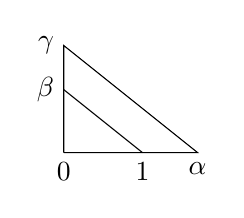
\begin{tikzpicture}[baseline=(Bs.base)]
		\node (Bs) at (0, 0.68) {};
		\draw (0,0) [below] node {$0$} -- (1.7, 0) [below] node {$\alpha$} -- (0, 1.36) [left] node {$\gamma$} -- (0,0);
		\draw (1,0) [below] node {$1$} -- (0, 0.8) [left] node {$\beta$};
	\end{tikzpicture}\]
	同理, 除法归结为正数相除的情形. 给定 $\gamma, \alpha > 0$, 上图亦说明如何构作 $\beta = \gamma/\alpha$. 

	已知如何平分 $\alpha \in \CC$ 的幅角, 平方根的构作归结为 $\alpha > 0$ 的情形. 请端详下图:
	\[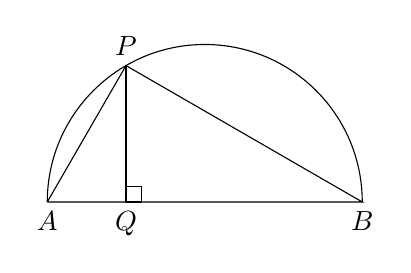
\begin{tikzpicture}[baseline=(Bs.base)]
		\node (Bs) at (90:1cm) {};
		\draw (0:2cm) arc [start angle=0, end angle=180, radius=2cm];
		\node (P) at (120:2cm) [above] {$P$};
		\draw (180:2cm) [below] node {$A$} -- (0:2cm) [below] node {$B$} -- (120:2cm) -- (180:2cm);
		\draw (120:2cm) -- (180:1cm) [below] node {$Q$};
		\draw (180:1cm) rectangle ++(0.2, 0.2);
	\end{tikzpicture} \quad |AQ|=1, \; |QB|=\alpha. \]
	根据相似形的性质导出 $|PQ|=\sqrt{\alpha}$. 最后, 共轭 $\alpha \mapsto \bar{\alpha}$ 无非是对实轴作镜射.
\end{proof}
此引理蕴涵 $\sqrt{-1} \in \text{Con}(\mathcal{S})$ 和
\[ z \in \text{Con}(\mathcal{S}) \iff \Re(z), \Im(z) \in \text{Con}(\mathcal{S}). \]

\begin{theorem}\label{prop:characterization-constructible}
	给定子集 $\{0, 1\} \subset \mathcal{S} \subset \CC$, 基于上述讨论不妨假定 $\mathcal{S}$ 对复共轭封闭, 它生成的子域记为 $\Q(\mathcal{S})$, 则复数 $z$ 满足 $z \in \mathrm{Con}(\mathcal{S})$ 当且仅当存在域扩张的塔
	\[ \Q(\mathcal{S}) = F_0 \subset F_1 \subset \cdots \subset F_n \subset \CC \]
	其中 $z \in F_n$, 而且对每个 $0 \leq i < n$ 皆有 $[F_{i+1} : F_i] = 2$. 特别地, $z$ 在 $\Q(\mathcal{S})$ 上代数.
\end{theorem}
易言之, 尺规作图的本领不多不少正是四则运算和取平方根.
\begin{proof}
	我们将运用一个性质: 若 $E = F_m$ 和 $E' = F'_n$ 皆是如上的二次扩张塔的末项, 则其复合 $EE'$ 亦然. 这点极易对 $\max\{n,m\}$ 递归地证明.

	设 $z$ 落在如上的 $F_n$ 中. 因为这里只涉及特征零的域, 二次扩张 $F_{i+1}|F_i$ 必为 $F_{i+1} = F_i(\sqrt{\alpha_i})$ 之形, $\alpha_i \in F_i^\times$. 配合引理 \ref{prop:ruler-compass-aux} 立得 $z \in F_n \subset \text{Con}(\mathcal{S})$. 反之令 $z \in \text{Con}(\mathcal{S})$. 回顾定义
	\[ \text{Con}(\mathcal{S}) = \bigcup_{k \geq 0} \mathcal{S}^{(k)}, \quad \mathcal{S}^0 = \mathcal{S}, \; \mathcal{S}^{(k+1)} = (\mathcal{S}^{(k)})'. \]
	给定一族点 $z_j = x_j + y_j \sqrt{-1} \in \mathcal{S}^{(k)}$ ($j=1,\ldots, m$), 并假设它们都落在同一个二次扩张塔 $\Q(\mathcal{S}) = F_0 \subset \cdots \subset F_n \subset \CC$ 中; 取复合后可假设 $F_n$ 对复共轭封闭. 从 $z_1, \ldots, z_m$ 出发作直线和圆, 其方程的系数都是 $x_j, y_j$ 的多项式, 因而也落在 $F_n$. 今探讨其间所有可能的交点, 分成实部虚部考虑:
	\begin{compactenum}[(a)]
		\item 线交线: 相当于解 $F_n$ 上的二元线性方程组, 不必扩张 $F_n$;
		\item 线交圆: 相当于解一个系数在 $F_n$ 里的二次方程, 交点坐标落在 $F_n$ 的二次扩张里;
		\item 圆交圆: 如交两点, 圆方程相减给出过交点的直线; 如切于一点则给出公切线. 化约到线交圆的情形.
	\end{compactenum}
	综之, $\mathcal{S}^{(k+1)}$ 的元素仍包含于二次扩张的塔. 证毕.
\end{proof}

作为推论, $z \in \text{Con}(\mathcal{S})$ 蕴涵 $[\Q(z, \mathcal{S}) : \Q(\mathcal{S})] \in 2^{\Z}$, 但其逆一般不真. 更完整的刻画可由 Galois 理论给出. 首先留意到定理 \ref{prop:characterization-constructible} 对 $z$ 的刻画与有根式解扩张的刻画 (定义 \ref{def:radical-ext} 和定理 \ref{prop:characterization-solvable-radicals}) 极为相近, 差异仅在于此处 $F_{i+1}$ 是由向 $F_i$ 添入平方根获得的, 条件更严. 这条性质同样可由群论刻画如下 (施于 $F = \Q(\mathcal{S}) \subset \CC$).
\begin{theorem}\label{prop:characterization-constructible-2}
	设域 $F$ 的特征 $\neq 2$ 而 $E|F$ 是可分有限扩张, 以下陈述等价.
	\begin{enumerate}[(i)]
		\item 存在二次域扩张的塔 $F = E_0 \subset \cdots \subset E_n$ 使得 $E \subset E_n$;
		\item 正规闭包 $E^\dagger|F$ 的 Galois 群是 $2$-群 (回顾定义 \ref{def:p-group}).
	\end{enumerate}
\end{theorem}
\begin{proof}
	重复定理 \ref{prop:characterization-solvable-radicals} 的论证可知 (i) 等价于 $G := \Gal(E^\dagger|F)$ 有合成列 $G = G_0 \supset \cdots \supset G_n = \{1\}$ 满足于 $G_i/G_{i+1} \simeq \Z/2\Z$, 特别地 $G$ 是 $2$-群; 此处由于 $\text{char}(F) \neq 2$, 不必再调用 Artin--Schreier 理论或添加单位根, 状况简化不少. 反之命题 \ref{prop:p-group-nilpotent} 蕴涵任意 $2$-群皆可解, 故具有如是合成列. 综上得 (i) $\iff$ (ii).
\end{proof}

I.\ M.\ Isaacs \cite{Is85} 发现一个有趣的相关结果: 设不可约多项式 $P \in \Q[X]$ 的所有根都是实数. 假设其中一根 $\alpha$ 可由实根式表达, 这相当于说存在定义 \ref{def:radical-ext} 中的塔 $\Q = E_0 \subset \cdots \subset E_n \ni \alpha$, 但要求 $E_n \subset \CC$ 且每一段 $E_{i+1}|E_i$ 添入的根都是实数, 那么 $\Gal(P)$ 是 $2$-群. 是故这类多项式的所有根都是尺规可构的.

对于最低要求 $\mathcal{S} = \{0,1\}$ 的情形, 域 $\text{Con} := \text{Con}(\mathcal{S})$ 由经典意义下所有尺规可构的复数组成. 现在可以处理曾令无数数学爱好者绞尽脑汁的古希腊三大作图难题. 代数方法说明它们在尺规的约束下一般无解.
\begin{description}
	\item[倍立方体] 给定边长 $a$ 的正立方体, 如何构作另一个正立方体使其体积加倍? 此处将构作正立方体理解为构作其边长. 问题等于是从 $\mathcal{S} = \{0, 1, a\}$ 出发构作 $b > 0$ 使得 $b^3 = 2a^3$. 取 $a=1$, 则 $[\Q(2^{1/3}):\Q] = 3 \notin 2^{\Z}$ 说明 $b$ 无法由尺规构作.
	
	\item[化圆为方] 给定一个圆, 能否以尺规构造一个面积等于圆面积的正方形? 同样可将问题理解为构造正方形的边长, 且可设圆半径为单位长 $1$, 问题遂化为以尺规构作 $\sqrt{\pi}$. 此问题的解答最终归结为 $\pi$ 的超越性.

	\item[三等分角] 给定平面上的角度 $\theta$, 求以尺规构造 $\theta/3$. 前面说过构作角度 $\theta$ 相当于构作单位圆上的 $\omega := e^{i\theta}$, 三等分角问题相当于从 $\mathcal{S} = \{0,1,\omega\}$ 出发构造 $\eta := e^{i\theta/3}$, $\eta^3 = \omega$. 为了说明一般而言 $\eta \notin \text{Con}(\mathcal{S})$, 以下取 $\theta := \pi/3$: 易见 $\omega = \frac{1 + \sqrt{-3}}{2} \in \text{Con}$, 问题归结为证明 $\eta \notin \text{Con}(\mathcal{S}) = \text{Con}$. 设若不然, 则 $\alpha := \Re(\eta) = \cos(\theta/3) \in \text{Con}$, 然而三倍角公式 $\cos(3x) = 4 \cos^3 x - 3\cos x$ 导致
	\[ 4\alpha^3 - 3\alpha - \cos\theta = 4\alpha^3 - 3\alpha - \frac{1}{2} = 0. \]
	代换 $\beta = 2\alpha$ 给出 $\beta^3 - 3\beta - 1 = 0$; 容易验证 $X^3 - 3X - 1 \in \Q[X]$ 无有理根故不可约. 于是由
	\[ [\Q(\alpha):\Q] = [\Q(\beta) : \Q] = 3 \notin 2^{\Z} \]
	知 $\alpha \notin \text{Con}$, 矛盾.
\end{description}

以上对三等分角的处理导向了同样经典的作图问题: 有哪些正 $n$ 边形可由尺规构造? 这个问题可以精确地表述为: 哪些 $n \in \Z_{\geq 1}$ 满足于 $\zeta_n := e^{\frac{2\pi i}{n}} \in \text{Con}$? (请读者思之)

我们需要以下概念: 形如 $p = 2^{2^a} + 1$ 之素数称为 Fermat 素数. 注意到 $A \geq 1$ 且 $2^A + 1$ 为素数蕴涵 $A = 2^a$, 这是因为若 $d$ 是 $A$ 的奇素因子, 则中学数学给出 $2^{A/d} + 1 \mid 2^A + 1$. 截至 \the\year 年, 已知的 Fermat 素数只有 $a=0,1,2,3,4$ 的情形.\index{Fermat 素数}

\begin{theorem}
	正整数 $n$ 满足 $\zeta_n \in \mathrm{Con}$ 当且仅当 $n$ 形如 $2^a p_1 \cdots p_k$, 其中 $p_1, \ldots, p_k$ 是相异的 Fermat 素数.
\end{theorem}
\begin{proof}
	应用定理 \ref{prop:characterization-constructible-2}, 问题归结为说明分圆扩张 $\Q(\zeta_n)|\Q$ 的 Galois 群 $G_n$ 何时为 $2$-群. 令 $n = \prod_{p: \text{素数}} p^{n_p}$, 中国剩余定理配合定理 \ref{prop:cyclotomic-Galois} 给出
	\[ G_n \simeq (\Z/n\Z)^\times \simeq \prod_{p: \text{素数}} (\Z/p^{n_p}\Z)^\times. \]
	原问题化为研究 $(\Z/p^m \Z)^\times$ 何时为 $2$-群. 由于该群有 $p^m - p^{m-1} = p^{m-1}(p-1)$ 个元素, 当 $p=2$ 时性质显然成立. 当 $p>2$ 时须要求 $m = 1$, 而且此时得到 $2$-群的充要条件是 $p-1 = 2^A$, 其中 $A \in \Z_{\geq 1}$. 此即等价于 $p$ 是 Fermat 素数.
\end{proof}

对于特例 $n = 17$, 正 17 边形的尺规作法是 Gauss 在 1796 年给出的, 详见 \cite[\S 29]{Har00}. 以上证明还有一个简单的变奏如下.
\begin{proposition}\label{prop:cos-rationality}
	设 $\theta \in \Q\pi$, 则 $\cos\theta$ 为有理数当且仅当 $\theta \in \left\{ \frac{\pi\Z}{2}, \frac{\pi\Z}{3} \right\}$.
\end{proposition}
由 $\sin\theta = \cos(\frac{\pi}{2} - \theta)$ 可推出 $\sin\theta$ 的情形, 兹不赘述.
\begin{proof}
	只需说明``仅当''方向. 若 $a := \cos\theta \in \Q$, 那么 $e^{i\theta} = \cos\theta + i\sin\theta \in \Q(i \sqrt{1 - a^2})$. 令 $\theta = \frac{2\pi m}{n}$, $(n,m)=1$, 则 $\Q(\zeta_n) = \Q(e^{i\theta})$ 成为 $\Q$ 的 $\leq 2$ 次扩张. 依旧利用 $\Gal(\Q(\zeta_n)|\Q) \simeq (\Z/n\Z)^\times$ 并考虑 $n$ 的素因子分解知此时必有 $n=2,3,4,6$, 可以逐一检验.
\end{proof}

% % % % % % % %
\begin{Exercises}
	\item 如果集合 $X$ 带有左 $\Gamma_F$-作用, 并且 $\Stab_{\Gamma_F}(x)$ 对每个 $x \in X$ 皆是 $\Gamma_F$ 的开子群, 则称 $X$ 为 $\Gamma_F$-集. 全体有限 $\Gamma_F$-集对等变映射构成范畴 $\Gamma_F\dcate{Set}$. 另一方面, 记 $F\dcate{EtAlg}$ 为全体平展 $F$-代数 (定义 \ref{def:etale-alg}) 所成范畴, 态射为 $F$-代数的同态. 证明 $\Gamma_F\dcate{Set}^\text{op}$ 同 $F\dcate{EtAlg}$ 等价.
	\begin{hint}
		定义函子 $\Theta: \Gamma_F\dcate{Set}^\text{op} \to F\dcate{EtAlg}$ 如下. 给定 $X$, 取 $\Theta(X)$ 为 $(F^\text{sep})^X$ 的 $\Gamma_F$-不动子代数. 等变映射 $f: Y \to X$ 自然地诱导 $f^*: (F^\text{sep})^X \to (F^\text{sep})^Y$, 进而导出 $\Theta(f)$. 拟逆函子可取为 $\Hom_{F\dcate{EtAlg}}(-, F^\text{sep})$.
	\end{hint}
	\item 设 $p$ 是素数, $\F_p \subset F$. 参照引理 \ref{prop:pins-polynomial} 的思路, 证明 $X^p - X - a \in F[X]$ 不可约当且仅当 $a \notin \left\{b^p -b : b \in F\right\}$; 证明此时 $F[X]/(X^p-X-a)$ 是 $F$ 的正规扩张.
	\item 设 $F$ 为特征 $p$ 的有限域, $n \geq 1$ 而 $f_1, \ldots, f_m \in F[X_1, \ldots, X_n]$. 假设它们的全次数满足
		\[ \deg f_1 + \cdots + \deg f_m < n. \]
		\begin{compactenum}[(i)]
			\item 证明 $f_1 = \cdots = f_m = 0$ 在 $F^n$ 中的解数 $\equiv 0 \pmod p$.
			\begin{hint}
				令 $q := |F|$, 那么解数 $\bmod\; p$ 同余 $\sum_{x \in F^n} \prod_{i=1}^m \left( 1 - f_i(x)^{q-1} \right)$; 此外 $0 \leq k < q-1 \implies \sum_{a \in F} a^k = 0$.
			\end{hint}
			\item 推出若 $(0, \ldots, 0)$ 是 $f_1 = \cdots = f_m = 0$ 的解 (例如当 $f_1, \ldots, f_m$ 皆齐次的情形), 则方程组必有一个不全为零的解.
		\end{compactenum}
		此结果称为 Chevalley--Warning 定理. 它联系到以下概念: 称域 $F$ 为 $C_1$ 的, 如果 $F$ 上变元数目超过全次数的齐次多项式皆有 $\neq (0, \ldots, 0)$ 的解. 因之有限域是 $C_1$ 域. 曾炯之首先研究了 $C_1$ 域, 相关性质可用于算术代数几何的研究.
	\item 对任意素数 $p$ 和正整数 $n$, 证明
		\[ \Phi_{pn}(X) = \begin{cases} \Phi_n(X^p), & p \mid n \\ \dfrac{\Phi_n(X^p)}{\Phi_n(X)}, & p \nmid n. \end{cases} \]
	\item 证明当 $n > 1$ 时分圆多项式 $\Phi_n$ 的常数项总是 $1$.
	\item 固定 $n \in \Z_{\geq 1}$, 证明:
		\begin{enumerate}[(i)]
			\item 设 $p$ 是素数, $p \nmid n$, 则存在 $a \in \Z$ 使得 $\Phi_n(a) \equiv 0 \pmod p$ 当且仅当 $a \bmod p$ 是 $(\Z/p\Z)^\times$ 中的 $n$ 阶元, 此时 $p \equiv 1 \pmod n$;
			\item 证明数列 $1 + n\Z_{\geq 1}$ 中有无穷多个素数; 这是 Dirichlet 定理的特例.
		\end{enumerate}
	\item 对分圆域 $\Q(\zeta_n)$ 证明 $\Q(\zeta_n) \cap \R = \Q\left( \zeta_n + \zeta_n^{-1} \right)$. 计算它对 $\Q$ 的扩张次数.
	\item 设 $p$ 为奇素数. 证明 $\Q(\zeta_p)$ 包含唯一的满足 $[E:\Q]=2$ 的子域 $E$, 而且 $E \subset \R$ 当且仅当 $p \equiv 1 \pmod{4}$.
	\item 以定理 \ref{prop:indep-character-Artin} 搭配定理 \ref{prop:norm-trace-field}, 重新证明可分扩张的迹型式 $(x,y) \mapsto \Tr_{E|F}(xy)$ 非退化.
	\item 确定 $\Q(\sqrt{2},\sqrt{3})$ 在 $\Q$ 上的次数, 描述 Galois 群并给出一组正规基.
	\item 证明 Galois 扩张 $E|F$ 是交换扩张当且仅当它的每个有限子扩张 $M|F$ 皆是交换扩张.
	\item 令 $D_1, \ldots, D_n$ 为两两互素的无平方因子整数. 令 $L := \Q(\sqrt{D_1}, \ldots, \sqrt{D_n})$. 以 Kummer 理论证明 $L|\Q$ 是 Galois 扩张, 且 $\Gal(L|\Q)$ 同构于 $(\Z/2\Z)^n$.
	\item 设 $P \in F[X]$ 为 $n \geq 1$ 次无重根多项式, 其根记为 $\alpha_1, \ldots, \alpha_n \in F^\text{sep}$, 分裂域记为 $L$. 回忆例 \ref{eg:polynomial-discriminant} 讨论的判别式 $\delta := \prod_{i < j} (\alpha_i - \alpha_j)^2$, 它是 $P$ 的系数之多项式, 而且无关根的排序. 设 $\mathrm{char}(F) \neq 2$.
		\begin{enumerate}[(i)]
			\item 证明 $\Gal(L|F) \cap \mathfrak{A}_n = \Gal\left( L \;|\; F(\sqrt{\delta}) \right)$;
			\item 在 $n=2, 3$ 的情形求 $\delta(P)$ 的公式, 据此给出判定三次多项式的 Galois 群的一套办法.
		\end{enumerate}
	\item 证明若子群 $H \subset \mathfrak{S}_p$ 含有一个对换和一个 $p$-循环 ($p$ 为素数), 则 $H = \mathfrak{S}_p$.
	\item 假设次数为素数 $p$ 的不可约多项式 $P \in \Q[X]$ 恰有 $p-2$ 个实根, 证明 $\Gal(P) = \mathfrak{S}_p$. 具体给出 $p=3$ 的例子.
	\item 以下探讨四次多项式 $P = X^4 - a_1 X^3 + a_2 X^2 -a_3 X^2 + a_4 \in F[X]$ 的 Galois 群, 此处设 $P$ 不可约而 $\text{char}(F) \neq 2$, 其分裂域记作 $L$.
		\begin{enumerate}[(i)]
			\item 证明 $F$ 上的四次不可约多项式皆无重根, 而且皆能化为以上形式.
			\item 设 $P$ 在 $L$ 里的根为 $x_1, \ldots, x_4$, 定义
				\begin{align*}
					u & := x_1 x_2 + x_3 x_4, \\
					v & := x_1 x_3 + x_2 x_4, \\
					w & := x_1 x_4 + x_2 x_3.
				\end{align*}
				将 $G := \Gal(L|F)$ 视为 $\mathfrak{S}_4$ 的子群, 证明 $F(u,v,w) = L^{G \cap V}$, 其中
				\[ V := \{1, (1 2)(3 4), (1 3)(2 4), (1 4)(2 3) \} \lhd \mathfrak{S}_4, \quad V \simeq (\Z/2\Z)^2. \]
			\item 证明
				\[ Q := (X-u)(X-v)(X-w) = X^3 - a_2 X^2 + (a_1 a_3 - 4a_4) X - (a_1^2 a_4 + a_3^2 - 4a_2 a_4), \]
				而且 $P, Q$ 有相同的判别式 $\delta \in F^\times$; 证明 $Q$ 的 Galois 群是 $G/G \cap V$. 一般称 $Q$ 为 $P$ 的三次预解式.
			\item 分类 $\mathfrak{S}_4$ 的传递子群:
				\begin{inparaenum}[(a)]
					\item $\mathfrak{S}_4$,
					\item $\mathfrak{A}_4$,
					\item $V$,
					\item $4$ 阶循环群 (两两共轭),
					\item Sylow $2$-子群 $\simeq D_8$ (两两共轭).
				\end{inparaenum}
			\item 建立下表:
				\[\begin{array}{c|c|c|c}
					\delta & Q \in F[X] & G & |G/G \cap V| \\ \hline\hline
					\notin F^{\times 2} & \text{不可约} & \mathfrak{S}_4 & 6 \\ \hline
					\in F^{\times 2} & \text{不可约} & \mathfrak{A}_4 & 3 \\ \hline
					\notin F^{\times 2} & \text{可约} & D_8\; \text{或}\; \Z/4\Z & 2 \\ \hline
					\in F^{\times 2} & \text{可约} & V & 1
				\end{array}\]
		\end{enumerate}
	\item 继续考虑上题中 $\delta \notin F^{\times 2}$ 而 $Q$ 可约的情形, 此时 $Q$ 的分裂域是 $F(\sqrt{\delta})$. 若 $P$ 在 $F(\sqrt{\delta})$ 上不可约则 $G \simeq D_8$, 否则 $G \simeq \Z/4\Z$. 然而这并不是唯一的区分方法.
	\item 补全定理 \ref{prop:characterization-constructible-2} 的证明.
	\item 有序域指的是一个域 $F$ 配上一个子集 $P \subset F$ (称为正锥), 满足于
		\begin{compactitem}
			\item $x, y \in P \implies x+y, xy \in P$;
			\item $F = P \sqcup \{0\} \sqcup (-P)$.
		\end{compactitem}
		证明
		\begin{compactenum}[(i)]
			\item 定义 $x < y \iff y-x \in P$ 将使 $(F, \leq)$ 成为全序集;
			\item $0 < x < y \implies x^{-1} > y^{-1} > 0$
			\item $x < y$, $z > 0$ 蕴涵 $xz < yz$;
			\item 任意平方和皆 $\geq 0$, 特别地 $\text{char}(F)=0$;
			\item $-1$ 不能表为平方和. 由此证明 $\CC$ 无法被赋予有序域结构.
		\end{compactenum}
	\item 假设有序域 $F$ 满足条件
		\begin{inparaenum}[(a)]
			\item $P = F^{\times\; 2}$ (因此序由 $F$ 的域结构完全确定);
			\item 任意奇数次 $Q \in F[X]$ 在 $F$ 中有根.
		\end{inparaenum}
		依序证明
		\begin{compactenum}[(i)]
			\item $F$ 的奇数次有限扩张只有 $F$ 本身;
			\item $\left[ F(\sqrt{-1}) : F \right]=2$ 且 $F(\sqrt{-1})$ 中任何元素皆有平方根;
			\item 应用引理 \ref{prop:alg-closed-decomp} 导出 $F(\sqrt{-1})$ 是代数闭域.
		\end{compactenum}
		\begin{hint}
			设 $Q \in F[X]$ 为不可约多项式, 令 $L|F$ 为 $Q \cdot (X^2+1)$ 的分裂域, $G := \Gal(L|F)$. 任何 Sylow $2$-子群 $H \subset G$ 皆给出奇数次扩张 $L^H | F$, 故 $G$ 是 $2$-群. 若子群 $\Gal\left( L|F(\sqrt{-1})\right)$ 非平凡, 则命题 \ref{prop:p-group-nilpotent} 和 Galois 对应将给出 $F(\sqrt{-1})$ 在 $L$ 中的 $2$ 次扩张, 矛盾; 若 $m=1$ 则必有 $L=F(\sqrt{-1})$.
		\end{hint}

		显然 $F=\R$ 满足条件 (a) 和 (b), 而 $\CC = \R(\sqrt{-1})$, 于是此题给出代数基本定理的又一证明, 习见的其它证明则更依赖于复变函数论等分析学工具. 此处并不是要尽量剥离非代数的成分, 用分析少者胜, 而在于这些条件确实有助于洞悉代数基本定理的底蕴, 并推至更广的情形. 满足条件 (a), (b) 的域 $F$ 称为\emph{实闭域}, 见 \cite[第 9 章]{Feng17}; Artin 和 Schreier 奠定了实闭域的一般理论, 见 \cite[Chapter XI]{Lang02}. 或许更值得一书的是: 实闭域可谓是模型论中 $o$-极小结构的先声, 后者在几何学中有出色应用. \index{moxinglun}
\end{Exercises}